% =====================================================================
%  Seminar: Introduction to RBF Approximation
%  Part 1 — Least-squares RBF approximation of scattered data
%  Examples: example01_rbf_mq_slsqp.py, example02_rbf_greedy_centers.py
%  Compile: pdflatex rbf_seminar_part1.tex   (twice)
% =====================================================================
\documentclass[10pt,aspectratio=169]{beamer}

\usetheme{metropolis}
\usepackage[utf8]{inputenc}
\usepackage[T1]{fontenc}
\usepackage{amsmath,amssymb,bm}
\usepackage{booktabs}
\usepackage{graphicx}
\usepackage{pgfplots}
\pgfplotsset{compat=1.16}
\usetikzlibrary{arrows.meta}
\usepackage{listings}
\usepackage[ruled,linesnumbered]{algorithm2e}
\usepackage{xcolor}

\graphicspath{{figures/}}

% ---- colors and small helpers ---------------------------------------
\definecolor{accent}{RGB}{200,60,40}
\definecolor{codebg}{RGB}{245,245,245}
\newcommand{\hl}[1]{\textcolor{accent}{\textbf{#1}}}
\newcommand{\R}{\mathbb{R}}
\newcommand{\x}{\bm{x}}
\newcommand{\cc}{\bm{c}}

\lstset{
  language=Python,
  basicstyle=\ttfamily\scriptsize,
  keywordstyle=\color{blue!70!black}\bfseries,
  commentstyle=\color{green!45!black}\itshape,
  stringstyle=\color{accent},
  backgroundcolor=\color{codebg},
  frame=single, rulecolor=\color{gray!40},
  showstringspaces=false, columns=fullflexible,
  xleftmargin=2pt, xrightmargin=2pt
}

% ---- title ----------------------------------------------------------
\title{Introduction to RBF Approximation}
\subtitle{Part 1 — Least-squares approximation of scattered data}
\author{Whady Felipe Florez}
\institute{Universidad Pontificia Bolivariana}
\date{}

\begin{document}

\maketitle

\begin{frame}{Point of view: two ways to approximate data}
  \centering
  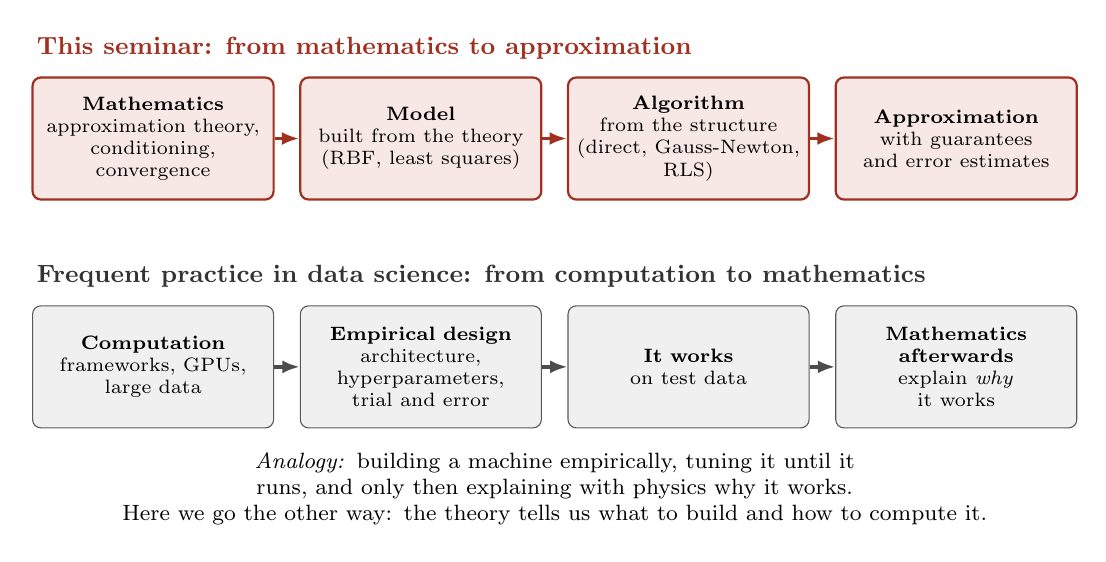
\begin{tikzpicture}[
      box/.style={draw, rounded corners=3pt, align=center, minimum height=1.55cm,
                  text width=2.85cm, font=\scriptsize, inner sep=3pt},
      ours/.style={box, fill=accent!12, draw=accent!80!black, thick},
      theirs/.style={box, fill=gray!12, draw=gray!70!black},
      arr/.style={-{Latex[length=2.2mm]}, very thick},
      lane/.style={font=\small\bfseries, anchor=west}]
    % ---- lane 1: this seminar -----------------------------------------
    \node[lane, text=accent!80!black] at (-1.6, 2.15)
      {This seminar: from mathematics to approximation};
    \node[ours] (m1) at (0,1)    {\textbf{Mathematics}\\approximation theory,\\conditioning,\\convergence};
    \node[ours] (m2) at (3.4,1)  {\textbf{Model}\\built from the theory\\(RBF, least squares)};
    \node[ours] (m3) at (6.8,1)  {\textbf{Algorithm}\\from the structure\\(direct, Gauss-Newton,\\RLS)};
    \node[ours] (m4) at (10.2,1) {\textbf{Approximation}\\with guarantees\\and error estimates};
    \draw[arr, accent!80!black] (m1) -- (m2);
    \draw[arr, accent!80!black] (m2) -- (m3);
    \draw[arr, accent!80!black] (m3) -- (m4);
    % ---- lane 2: frequent practice ------------------------------------
    \node[lane, text=gray!40!black] at (-1.6, -0.75)
      {Frequent practice in data science: from computation to mathematics};
    \node[theirs] (c1) at (0,-1.9)    {\textbf{Computation}\\frameworks, GPUs,\\large data};
    \node[theirs] (c2) at (3.4,-1.9)  {\textbf{Empirical design}\\architecture,\\hyperparameters,\\trial and error};
    \node[theirs] (c3) at (6.8,-1.9)  {\textbf{It works}\\on test data};
    \node[theirs] (c4) at (10.2,-1.9) {\textbf{Mathematics afterwards}\\explain \emph{why}\\it works};
    \draw[arr, gray!60!black] (c1) -- (c2);
    \draw[arr, gray!60!black] (c2) -- (c3);
    \draw[arr, gray!60!black] (c3) -- (c4);
    % ---- the analogy ---------------------------------------------------
    \node[font=\footnotesize, align=center, text width=13cm] at (5.1,-3.45)
      {\emph{Analogy:} building a machine empirically, tuning it until it runs,
       and only then explaining with physics why it works.\\
       Here we go the other way: the theory tells us what to build and how
       to compute it.};
  \end{tikzpicture}
\end{frame}

\begin{frame}
\centering
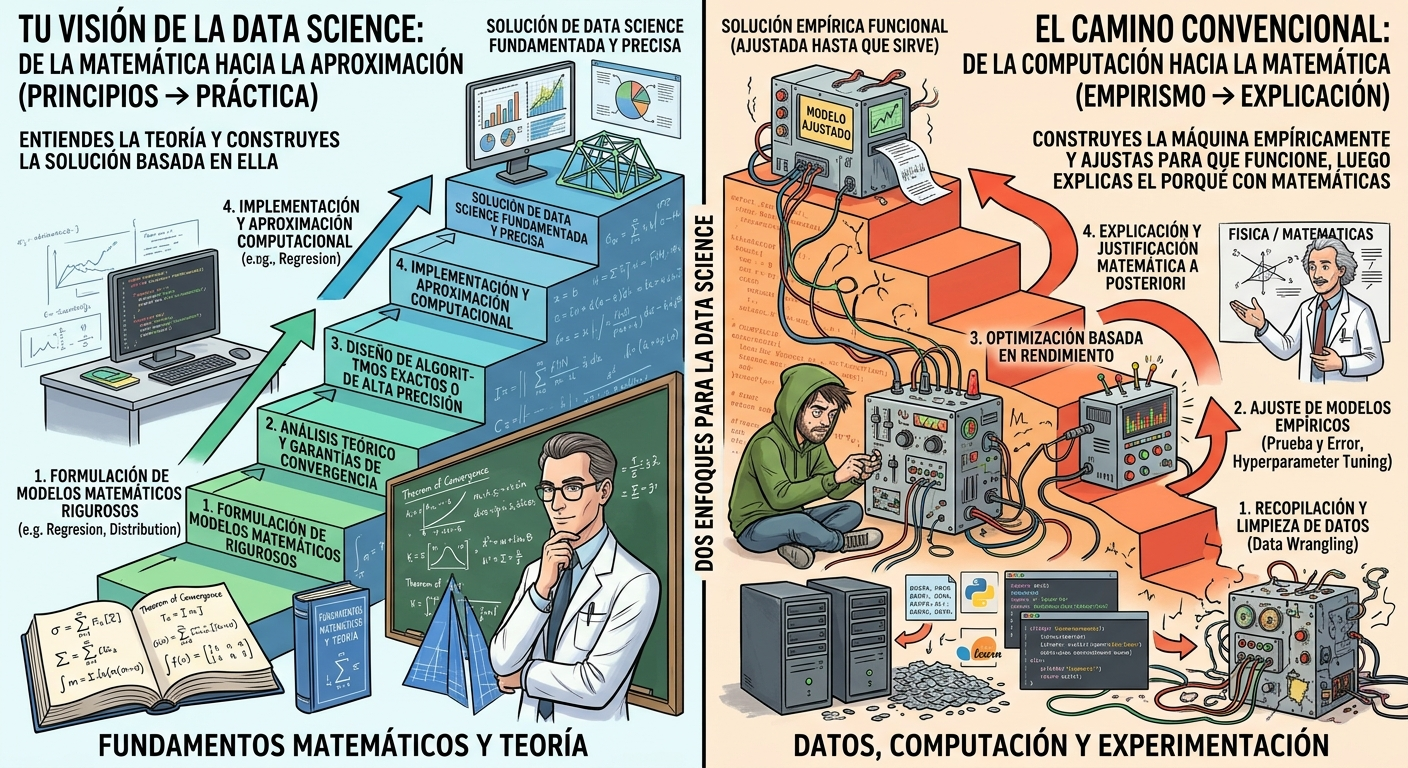
\includegraphics[width=\linewidth,height=0.80\textheight,keepaspectratio]{irony.jpg}
\end{frame}

\begin{frame}{Outline}
  \begin{columns}[T]
    \begin{column}{0.48\textwidth}
      \tableofcontents[sections={1-5}]
    \end{column}
    \begin{column}{0.48\textwidth}
      \tableofcontents[sections={6-10}]
    \end{column}
  \end{columns}
\end{frame}

% =====================================================================
\section{The problem}
% =====================================================================

\begin{frame}{What we have: scattered data}
  \begin{columns}[T]
    \begin{column}{0.48\textwidth}
      We are given $n$ measurements
      \[
        (\x_i,\, y_i), \qquad \x_i \in \R^2,\quad i=1,\dots,n
      \]
      \begin{itemize}
        \item The points $\x_i$ are \hl{scattered}: no grid, no structure.
        \item The values are $y_i = f(\x_i) + \text{noise}$.
        \item The function $f$ is \hl{unknown}.
      \end{itemize}
      \vspace{0.3em}
      \textbf{Goal:} build a function $s(\x)$, defined \emph{everywhere},
      that represents the data well.
    \end{column}
    \begin{column}{0.50\textwidth}
      \centering
      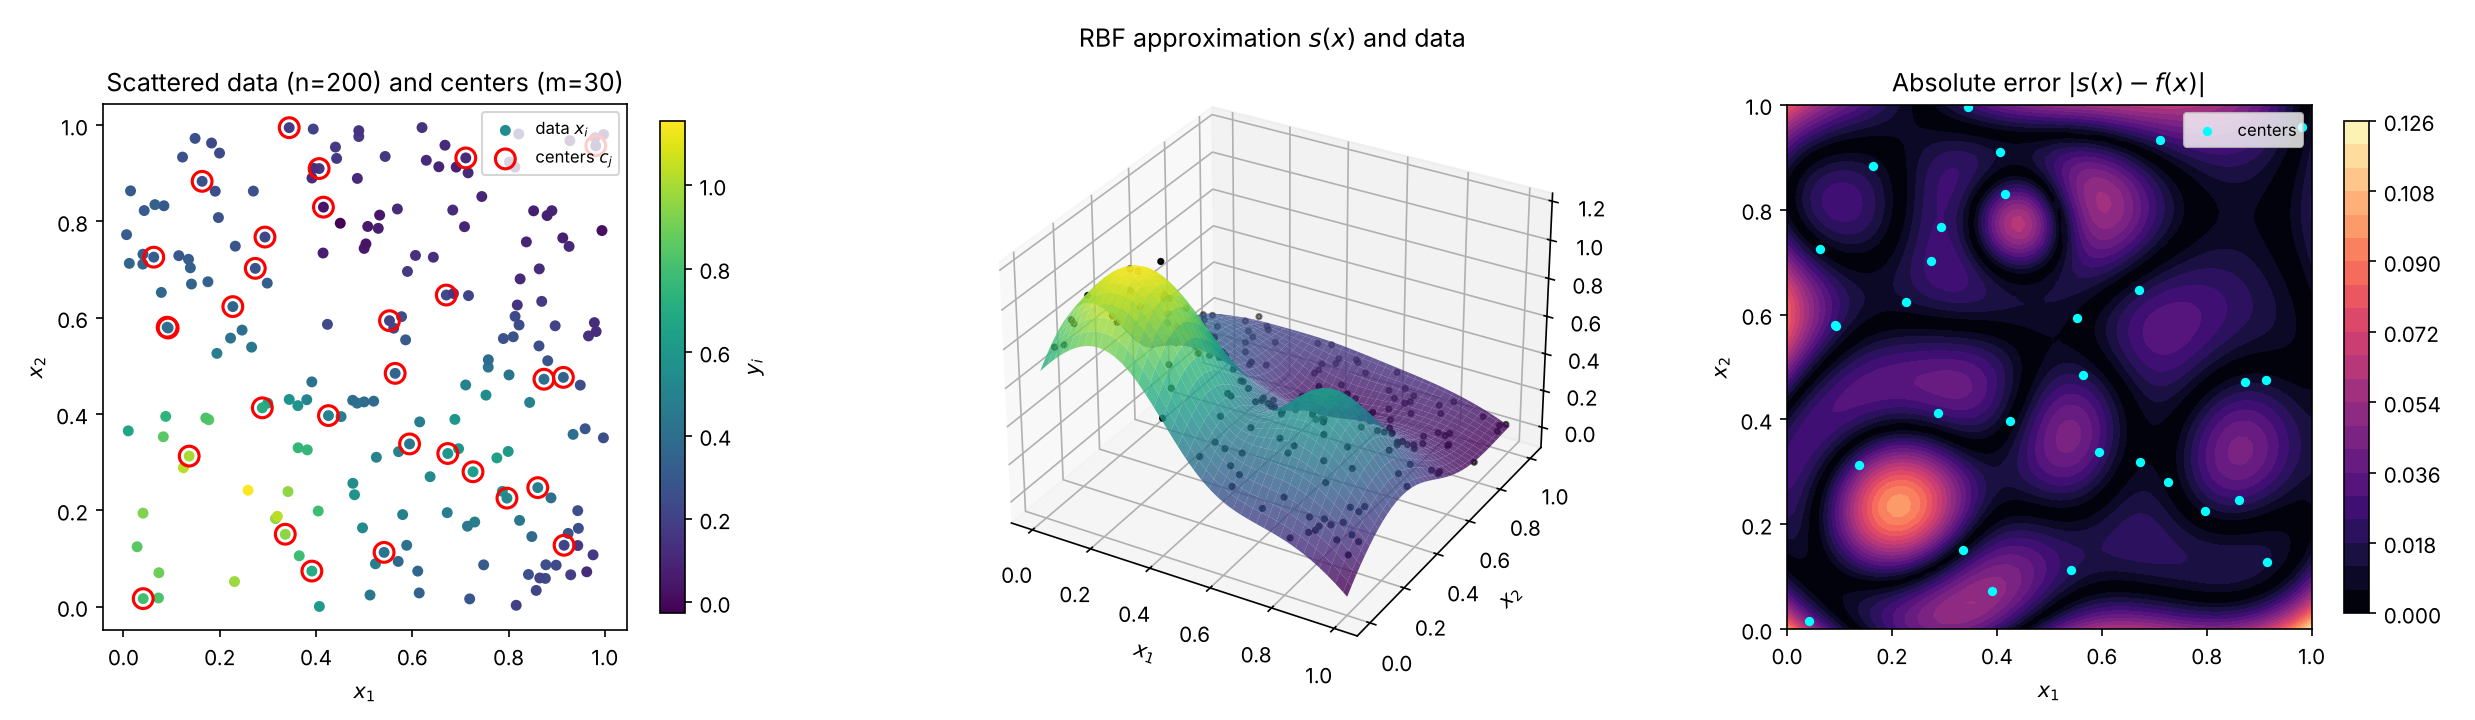
\includegraphics[height=0.72\textheight,trim=0 0 766 0,clip]{example01_results.png}
    \end{column}
  \end{columns}
\end{frame}

\begin{frame}{Interpolation or approximation?}
  \begin{columns}[T]
    \begin{column}{0.48\textwidth}
      \textbf{Interpolation}
      \begin{itemize}
        \item $s(\x_i) = y_i$ \emph{exactly}, for every $i$.
        \item As many unknowns as data: $n$ equations, $n$ unknowns.
        \item Reproduces the \hl{noise} too.
        \item Large $n$ $\Rightarrow$ large, often ill-conditioned systems.
      \end{itemize}
    \end{column}
    \begin{column}{0.48\textwidth}
      \textbf{Approximation} (this seminar)
      \begin{itemize}
        \item $s(\x_i) \approx y_i$.
        \item Few unknowns: $m < n$ terms.
        \item More equations than unknowns $\Rightarrow$ solve in the
              \hl{least-squares} sense.
        \item Smooths the noise, cheaper model.
      \end{itemize}
    \end{column}
  \end{columns}
  \vspace{1em}
  \begin{alertblock}{Key question}
    Which $m$ terms should we use, and how do we compute their coefficients?
  \end{alertblock}
\end{frame}

% =====================================================================
\section{The RBF model}
% =====================================================================

\begin{frame}{Radial basis functions}
  \begin{columns}[c]
    \begin{column}{0.50\textwidth}
      A \hl{radial} function depends only on the \emph{distance} to a point
      $\cc$, called its \textbf{center}:
      \[
        \phi\big(\lVert \x - \cc \rVert\big)
      \]
      \begin{itemize}
        \item Works in any dimension: only distances are needed.
        \item No mesh, no grid: ideal for scattered data.
      \end{itemize}
      \vspace{0.3em}
      \textbf{Multiquadric (MQ):}
      \[
        \phi(r) = \sqrt{1 + (\varepsilon r)^2}
      \]
      $\varepsilon > 0$ is the \hl{shape parameter}.
    \end{column}
    \begin{column}{0.48\textwidth}
      \centering
      \begin{tikzpicture}
        \begin{axis}[
          width=\linewidth, height=0.62\textheight,
          xlabel={$r = \lVert \x - \cc\rVert$}, ylabel={$\phi(r)$},
          xmin=-1, xmax=1, ymin=0, ymax=6.5,
          legend pos=north west, legend style={font=\scriptsize},
          tick label style={font=\scriptsize}, label style={font=\small},
          samples=101, domain=-1:1, thick]
          \addplot[blue]   {sqrt(1+(1*x)^2)};  \addlegendentry{$\varepsilon=1$}
          \addplot[accent] {sqrt(1+(3*x)^2)};  \addlegendentry{$\varepsilon=3$}
          \addplot[green!50!black] {sqrt(1+(6*x)^2)}; \addlegendentry{$\varepsilon=6$}
        \end{axis}
      \end{tikzpicture}

      {\scriptsize Small $\varepsilon$: flat. Large $\varepsilon$: sharp ``V''.}
    \end{column}
  \end{columns}
\end{frame}

\begin{frame}{Polynomial augmentation}
  We add a low-degree polynomial to the RBF sum. In 2D, a quadratic
  polynomial has \hl{6 terms}:
  \[
    p_k(\x) \in \{\,1,\; x_1,\; x_2,\; x_1^2,\; x_1x_2,\; x_2^2\,\}
  \]
  \textbf{Why?}
  \begin{itemize}
    \item The model can reproduce smooth trends (constants, slopes,
          curvature) exactly.
    \item Better accuracy, especially near the boundary of the domain.
    \item The RBFs only have to capture what the polynomial cannot.
  \end{itemize}
  \vspace{0.5em}
  \begin{block}{The complete model with $m$ centers}
    \[
      s(\x) \;=\; \underbrace{\sum_{j=1}^{m} a_j\,
        \phi\big(\lVert \x - \cc_j \rVert\big)}_{\text{RBF part}}
      \;+\; \underbrace{\sum_{k=1}^{6} b_k\, p_k(\x)}_{\text{polynomial part}}
    \]
    Unknowns: $a_1,\dots,a_m$ and $b_1,\dots,b_6$ \;$\Rightarrow$\; $m+6$ coefficients.
  \end{block}
\end{frame}

\begin{frame}{The model in matrix form}
  Evaluating $s$ at the $n$ data points gives $n$ equations
  $s(\x_i) \approx y_i$, i.e.
  \[
    \underbrace{\begin{bmatrix} \Phi & P \end{bmatrix}}_{A\;(n\times(m+6))}
    \underbrace{\begin{bmatrix} \bm{a} \\ \bm{b} \end{bmatrix}}_{\bm{w}}
    \;\approx\; \bm{y},
    \qquad
    \Phi_{ij} = \phi\big(\lVert \x_i - \cc_j\rVert\big), \quad
    P_{ik} = p_k(\x_i)
  \]
  \begin{itemize}
    \item Row $i$ $\leftrightarrow$ data point $\x_i$.
    \item Column $j$ of $\Phi$ $\leftrightarrow$ RBF centered at $\cc_j$.
    \item $n > m+6$: \hl{overdetermined} system, no exact solution in general.
  \end{itemize}
  \vspace{0.3em}
  \begin{block}{Least squares}
    Choose $\bm{w}$ that minimizes the total squared error
    \[
      \text{SSE} = \sum_{i=1}^{n} \big(s(\x_i) - y_i\big)^2
                 = \lVert A\bm{w} - \bm{y} \rVert^2
    \]
  \end{block}
\end{frame}

\begin{frame}{The orthogonality condition}
  With polynomial augmentation it is usual to impose
  \[
    \sum_{j=1}^{m} a_j\, p_k(\cc_j) = 0, \quad k=1,\dots,6
    \qquad\Longleftrightarrow\qquad
    P_c^{T}\bm{a} = \bm{0}
  \]
  where $P_c$ is the polynomial matrix evaluated at the \emph{centers}.
  \vspace{0.5em}
  \begin{itemize}
    \item It prevents the RBF part from ``imitating'' the polynomial part:
          each part has its own job.
    \item In \hl{interpolation} ($m = n$) it is \emph{necessary}: it gives the
          6 extra equations that make the square system uniquely solvable.
    \item In \hl{approximation} ($m < n$) it is \emph{optional}: least squares
          already has a unique solution if $A$ has full rank.
  \end{itemize}
  \vspace{0.5em}
  We will use it in Example~1, and discuss when to drop it in Example~2.
\end{frame}

% =====================================================================
\section{Example 1: random centers}
% =====================================================================

\begin{frame}[fragile]{Example 1: setup}
  \begin{columns}[T]
    \begin{column}{0.52\textwidth}
      \begin{itemize}
        \item True function: \hl{Franke's function}, a classical test function
              on $[0,1]^2$ (unknown in practice).
        \item $n = 200$ random points, noise $\sigma = 0.02$.
        \item $m = 30$ centers, chosen \hl{at random} among the data points.
        \item MQ with \emph{fixed} $\varepsilon = 3$.
        \item Quadratic polynomial (6 terms).
      \end{itemize}
      \vspace{0.3em}
      Unknowns: $m + 6 = 36$ \quad Equations: $n = 200$
    \end{column}
    \begin{column}{0.44\textwidth}
\begin{lstlisting}
SEED      = 0
N_DATA    = 200
M_CENTERS = 30
EPS       = 3.0
NOISE     = 0.02

X = rng.random((N_DATA, 2))
y = franke(X[:,0], X[:,1]) \
    + NOISE*rng.standard_normal(N_DATA)

idx = rng.choice(N_DATA, M_CENTERS,
                 replace=False)
C = X[idx]           # the centers
\end{lstlisting}
    \end{column}
  \end{columns}
\end{frame}

\begin{frame}[fragile]{Example 1: the optimization problem}
  \[
    \min_{\bm{w}}\; J(\bm{w}) = \tfrac12\,\lVert A\bm{w} - \bm{y}\rVert^2
    \qquad \text{subject to} \qquad P_c^T\bm{a} = \bm{0}
  \]
  \begin{columns}[T]
    \begin{column}{0.46\textwidth}
      \begin{itemize}
        \item Exact gradient:
              $\nabla J = A^T(A\bm{w} - \bm{y})$.
        \item Solver: \texttt{scipy.optimize.minimize} with \hl{SLSQP}
              (Sequential Least-Squares Quadratic Programming).
        \item SLSQP accepts \hl{equality constraints}; BFGS and similar
              methods do not.
      \end{itemize}
    \end{column}
    \begin{column}{0.52\textwidth}
\begin{lstlisting}
def J(w):
    r = A @ w - y
    return 0.5 * r @ r

def grad_J(w):
    return A.T @ (A @ w - y)

G = np.hstack([Pc.T, np.zeros((6, 6))])
cons = [{"type": "eq",
         "fun": lambda w: G @ w,
         "jac": lambda w: G}]

sol = minimize(J, np.zeros(n_par),
               jac=grad_J, constraints=cons,
               method="SLSQP")
\end{lstlisting}
    \end{column}
  \end{columns}
\end{frame}

\begin{frame}{Example 1: results}
  \centering
  \begin{tabular}{lr}
    \toprule
    Quantity & Value \\
    \midrule
    SLSQP converged & yes, 248 iterations \\
    Constraint residual $\lVert P_c^T\bm{a}\rVert$ & $\approx 10^{-13}$ \\
    Condition number $\operatorname{cond}(A)$ & $2.7\times 10^{6}$ \\
    \midrule
    Total squared error $\sum_i (s(\x_i)-y_i)^2$ & $0.132$ \\
    RMSE at the data points & $0.026$ \\
    RMSE vs.\ true $f$ on an $80\times80$ grid & $0.027$ \\
    Maximum error on the grid & $0.121$ \\
    \bottomrule
  \end{tabular}
  \vspace{1em}

  \small The RMSE is of the order of the noise level $\sigma = 0.02$:
  the model captures $f$, not the noise.
\end{frame}

\begin{frame}{Example 1: the approximated surface}
  \begin{columns}[c]
    \begin{column}{0.58\textwidth}
      \centering
      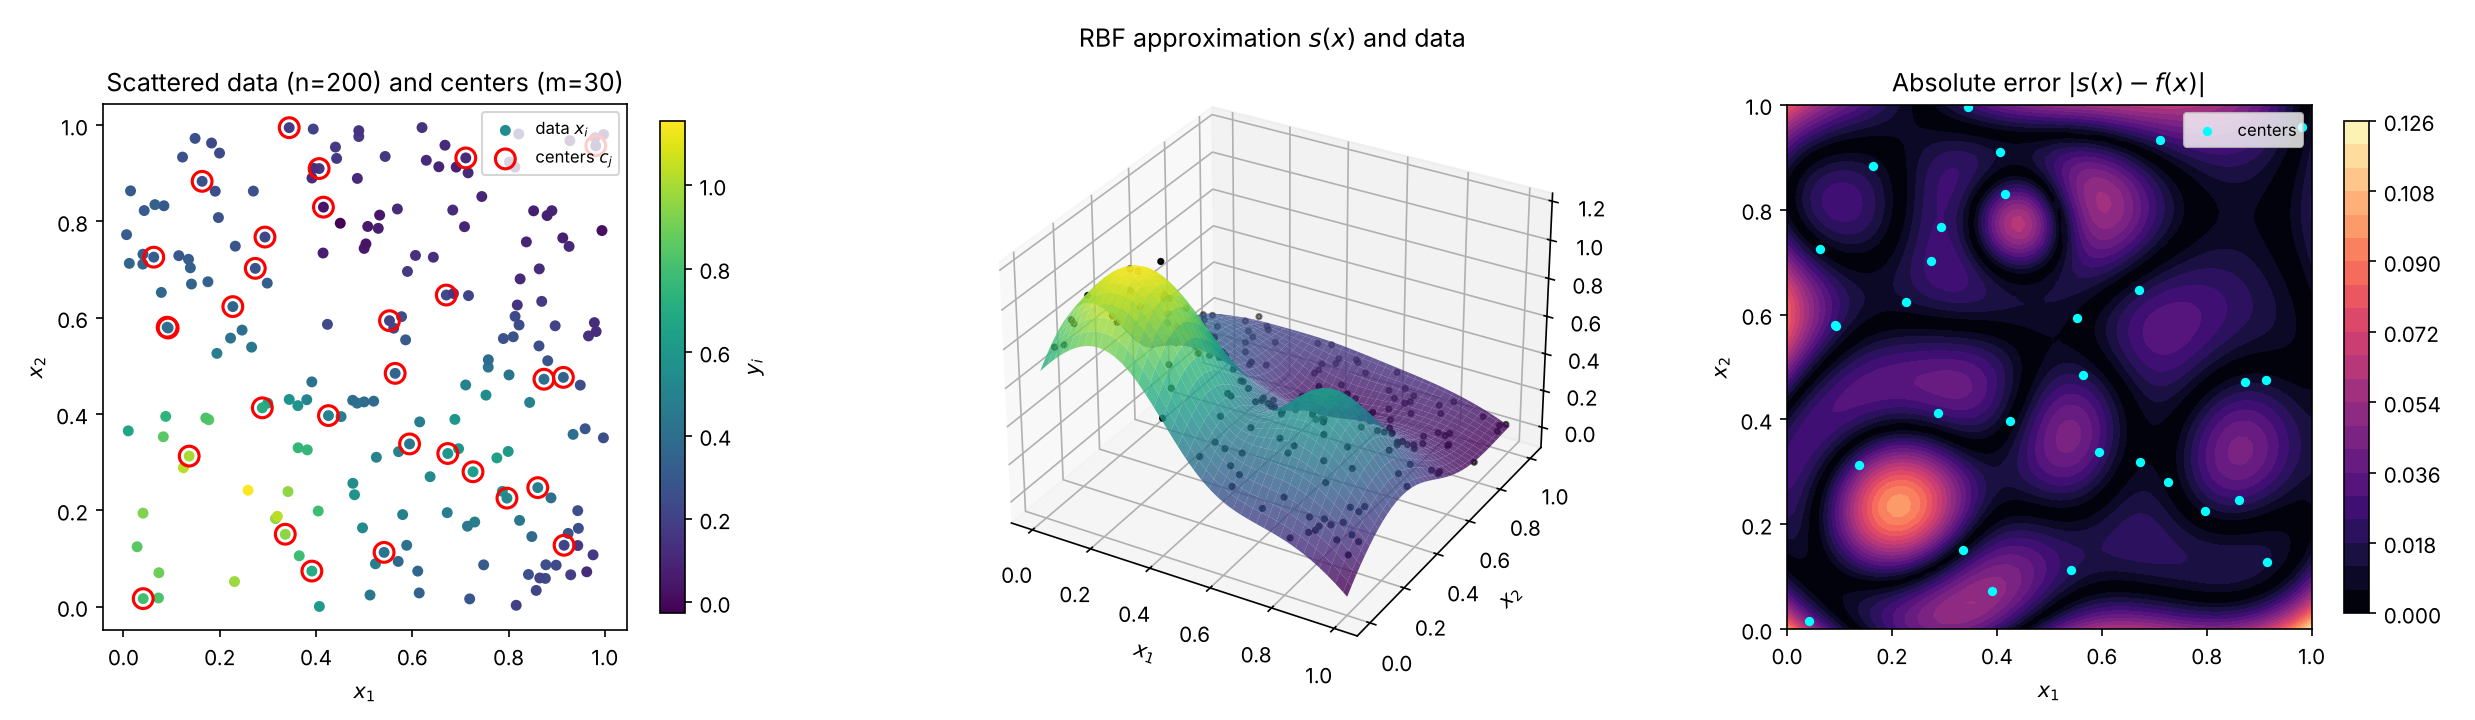
\includegraphics[width=\linewidth,height=0.80\textheight,keepaspectratio,trim=422 0 391 0,clip]{example01_results.png}
    \end{column}
    \begin{column}{0.40\textwidth}
      \begin{itemize}
        \item Surface: $s(\x)$ evaluated on a fine grid.
        \item Black dots: the 200 noisy data $y_i$.
        \item The surface follows the trend of the data without passing exactly through each point.
      \end{itemize}
    \end{column}
  \end{columns}
\end{frame}

\begin{frame}{Example 1: where is the error?}
  \begin{columns}[c]
    \begin{column}{0.58\textwidth}
      \centering
      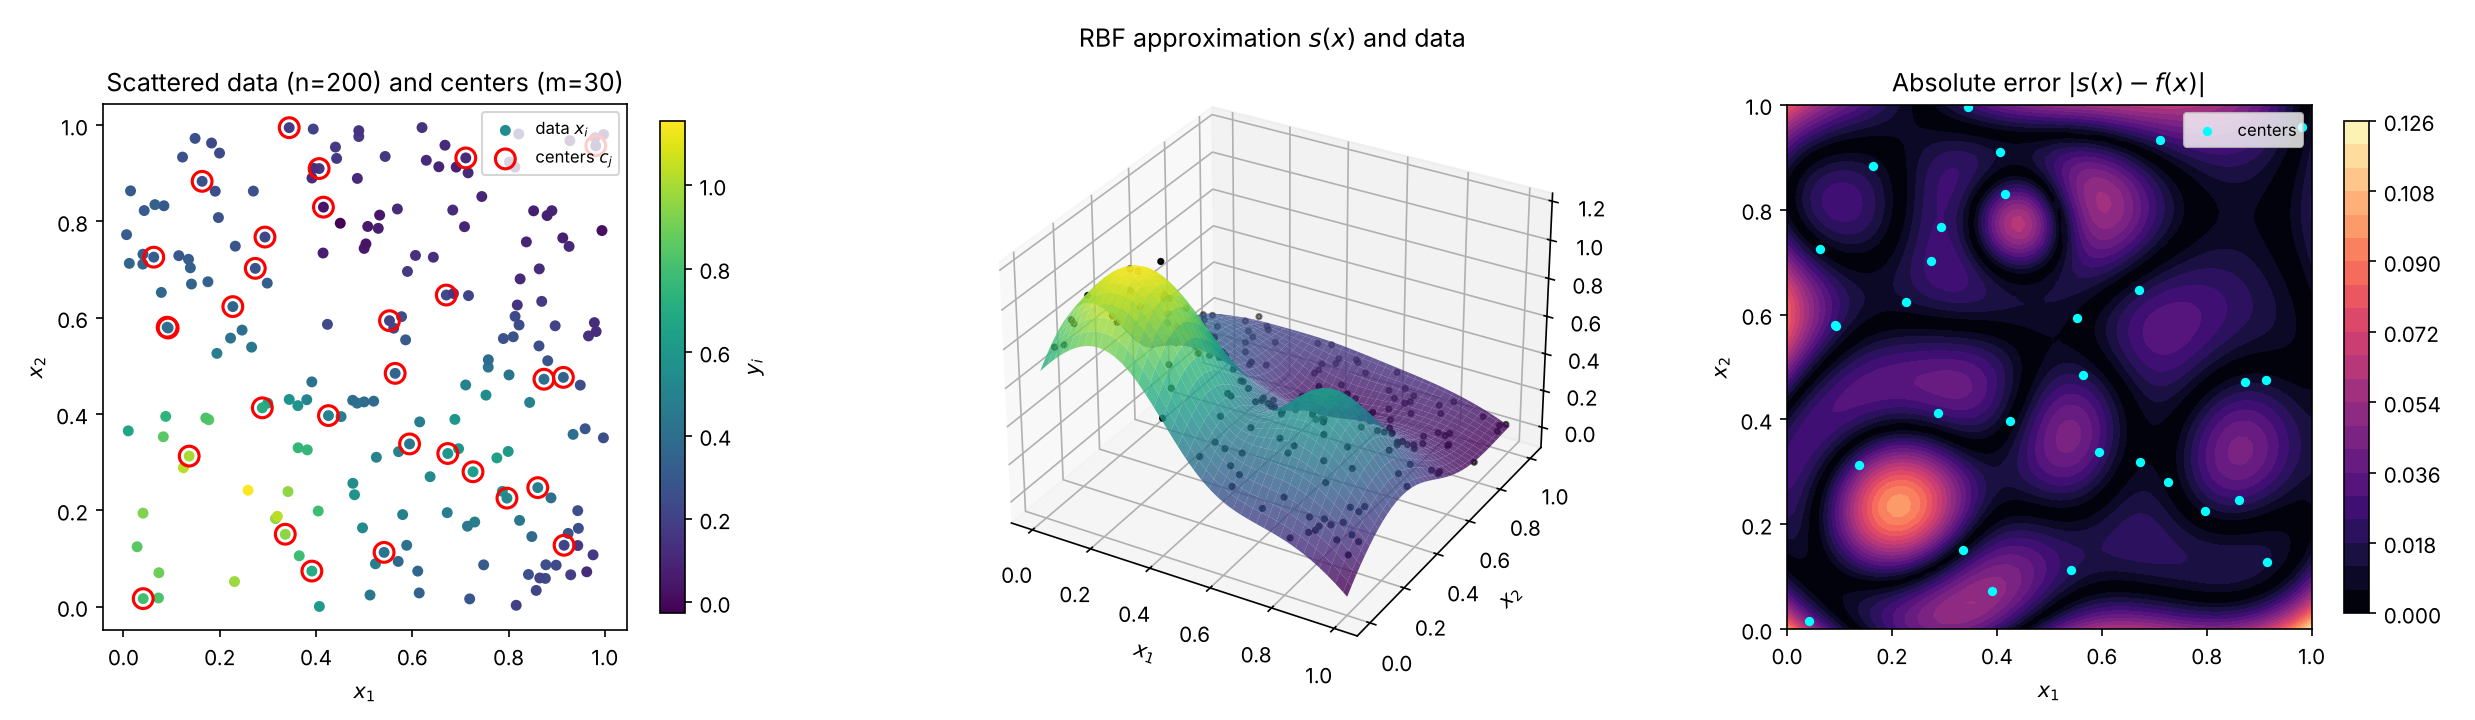
\includegraphics[width=\linewidth,height=0.80\textheight,keepaspectratio,trim=797 0 0 0,clip]{example01_results.png}
    \end{column}
    \begin{column}{0.40\textwidth}
      \begin{itemize}
        \item Color: $|s(\x)-f(\x)|$, computed only because we know $f$.
        \item Cyan dots: the 30 random centers.
        \item Largest errors: near the corners and around the peak at $\approx(0.2,0.2)$, where $f$ changes fast.
        \item Some regions get several centers, others almost none.
      \end{itemize}
    \end{column}
  \end{columns}
\end{frame}

\begin{frame}{Example 1: observations}
  \begin{enumerate}
    \item \textbf{Approximation works:} 36 coefficients represent 200 noisy
          values with an error close to the noise level.
    \item \textbf{The error is not uniform.} It is larger where the function
          varies fast and where there are few centers (e.g.\ near the
          corners and around the peak at $\approx(0.2,0.2)$).
    \item \textbf{Ill-conditioning.} $\operatorname{cond}(A)\sim 10^6$: many
          different coefficient vectors give almost the same fit. The fit
          is reliable; individual coefficients are not.
    \item \textbf{SLSQP is slow here.} The problem is quadratic, but SLSQP
          builds a quasi-Newton approximation of the Hessian ($A^TA$), so it
          needs $\sim 250$ iterations.
  \end{enumerate}
\end{frame}

\begin{frame}{An alternative formulation}
  The orthogonality conditions can also be written as \hl{extra equations}
  of the collocation system:
  \[
    \begin{bmatrix} \Phi & P \\ P_c^T & 0 \end{bmatrix}
    \begin{bmatrix} \bm{a} \\ \bm{b} \end{bmatrix}
    \approx
    \begin{bmatrix} \bm{y} \\ \bm{0} \end{bmatrix}
    \qquad \big((n+6)\times(m+6)\big)
  \]
  \begin{itemize}
    \item One overdetermined system, solved in the optimal (least-squares)
          sense, e.g.\ with iterative methods (LSQR, LSMR).
    \item Difference: the constraint is satisfied only
          \emph{approximately}, competing with the data residuals.
    \item To enforce it more strongly, multiply the last 6 rows by a large
          weight.
  \end{itemize}
\end{frame}

% =====================================================================
\section{Example 2: greedy selection of centers}
% =====================================================================

\begin{frame}{Motivation}
  In Example 1 the centers were chosen at random. Look at the figure:
  \begin{itemize}
    \item Some regions have several centers close together.
    \item Other regions, where $f$ changes fast, have few or none.
  \end{itemize}
  \vspace{0.5em}
  \begin{alertblock}{Question}
    Can we choose the centers \emph{using the data}, so that each center is
    placed where it helps most?
  \end{alertblock}
  \vspace{0.5em}
  \textbf{Idea (greedy):} add centers one at a time. At each step, try every
  candidate and keep the one that reduces the error the most.
\end{frame}

\begin{frame}{The greedy algorithm}
  \begin{columns}[c]
    \begin{column}{0.64\textwidth}
      \footnotesize
      \begin{algorithm}[H]
        \caption{Greedy center selection}
        $S \leftarrow \emptyset$ \tcp*{polynomial-only model}
        $\text{SSE}_0 \leftarrow$ least-squares error with $S$\;
        \For{$k = 1, 2, \dots$}{
          \ForEach{data point $\cc \notin S$}{
            $A \leftarrow [\,\Phi(X, S\cup\{\cc\}) \mid P(X)\,]$\;
            solve $\min_{\bm{w}} \lVert A\bm{w}-\bm{y}\rVert^2$\;
            $\text{SSE}(\cc) \leftarrow \lVert A\bm{w}-\bm{y}\rVert^2$\;
          }
          $\cc^\ast \leftarrow \arg\min_{\cc}\, \text{SSE}(\cc)$\;
          \If{$(\text{SSE}_{k-1}-\text{SSE}(\cc^\ast))/\text{SSE}_{k-1} < \text{TOL}$}{
            \textbf{stop} \tcp*{$\cc^\ast$ is rejected}
          }
          $S \leftarrow S \cup \{\cc^\ast\}$,\;
          $\text{SSE}_k \leftarrow \text{SSE}(\cc^\ast)$\;
        }
        Final refit with $S$ \textbf{and} $P_c^T\bm{a}=\bm{0}$ (SLSQP)\;
      \end{algorithm}
    \end{column}
    \begin{column}{0.34\textwidth}
      \begin{itemize}
        \item Candidates: all $n$ data points.
        \item Step $k$ tries $n-(k-1)$ candidates.
        \item Same data, $\varepsilon$ and polynomial as Example~1.
      \end{itemize}
    \end{column}
  \end{columns}
\end{frame}

\begin{frame}{Design decision 1: no constraint during the selection}
  With $k$ centers, $P_c^T\bm{a} = \bm{0}$ is a system of
  \hl{6 equations with $k$ unknowns}.
  \begin{itemize}
    \item If $k < 6$, in general the only solution is $\bm{a} = \bm{0}$.
    \item Every candidate would give the same error (polynomial only)
          $\Rightarrow$ the greedy algorithm could not even start.
  \end{itemize}
  \vspace{0.5em}
  \textbf{Solution:}
  \begin{itemize}
    \item \textbf{Selection:} RBF + polynomial, \emph{without} constraint
          (allowed: the problem is overdetermined, $k+6 < n$).
    \item \textbf{Final refit:} with the selected centers, RBF + polynomial
          \emph{with} constraint, solved with SLSQP exactly as in Example 1.
  \end{itemize}
\end{frame}

\begin{frame}[fragile]{Design decision 2: a fast solver for the trial fits}
  \begin{itemize}
    \item The greedy loop needs \hl{thousands} of least-squares fits
          (here $\approx 7000$).
    \item SLSQP is iterative ($\sim$250 iterations per fit): far too slow.
    \item \texttt{scipy.linalg.lstsq} solves each fit \hl{directly}
          (SVD), in one step.
    \item Trick: every candidate is a data point, so we compute
          \emph{once} the $n\times n$ matrix
          $\Phi_{\text{all}}[i,j] = \phi(\lVert \x_i - \x_j\rVert)$ and just
          pick columns.
  \end{itemize}
\begin{lstlisting}
Phi_all = multiquadric(distances(X, X), EPS)     # n x n, computed once

def ls_fit(idx):
    A = np.hstack([Phi_all[:, idx], P_data])     # n x (k+6)
    w, *_ = lstsq(A, y)
    r = A @ w - y
    return w, r @ r                              # coefficients, SSE
\end{lstlisting}
\end{frame}

\begin{frame}{Stopping criterion}
  Stop when one more center \hl{no longer helps enough}:
  \[
    \frac{\text{SSE}_{k-1} - \text{SSE}_k}{\text{SSE}_{k-1}} < \text{TOL}
    \qquad (\text{TOL} = 1\%)
  \]
  A cap $M_{\max} = n/2$ only protects against an endless loop (not reached).
  \vspace{0.5em}

  \centering\small
  \begin{tabular}{lll}
    \toprule
    Level & What it does & Stopping criterion? \\
    \midrule
    Outer greedy loop & adds centers one by one & yes: relative improvement $<$ TOL \\
    Inner loop & tries all remaining candidates & no: ends when the list ends \\
    Each trial fit & \texttt{lstsq} (direct) & no: not iterative \\
    Final refit & SLSQP with constraint & yes: SLSQP's own tolerance \\
    \bottomrule
  \end{tabular}
\end{frame}

\begin{frame}{Example 2: results}
  The greedy loop stopped at \hl{$m = 39$ centers}: the 40th best candidate
  improved the SSE by only $0.43\%$. Total: $\approx 7000$ trial fits in
  about 2 seconds.
  \vspace{0.8em}

  \centering
  \begin{tabular}{lcc}
    \toprule
    Model ($m = 39$) & Total squared error & RMSE vs.\ true $f$ \\
    \midrule
    Greedy, without constraint & $0.052$ & $0.019$ \\
    Greedy, with constraint (SLSQP) & $0.068$ & $0.018$ \\
    Random, with constraint (SLSQP) & $0.094$ & $0.021$ \\
    \bottomrule
  \end{tabular}
  \vspace{0.8em}

  \raggedright\small
  Removing the constraint lowers the error \emph{on the data}, but the
  error against the true function is practically the same.
\end{frame}

\begin{frame}{Example 2: the selected centers}
  \begin{columns}[c]
    \begin{column}{0.55\textwidth}
      \centering
      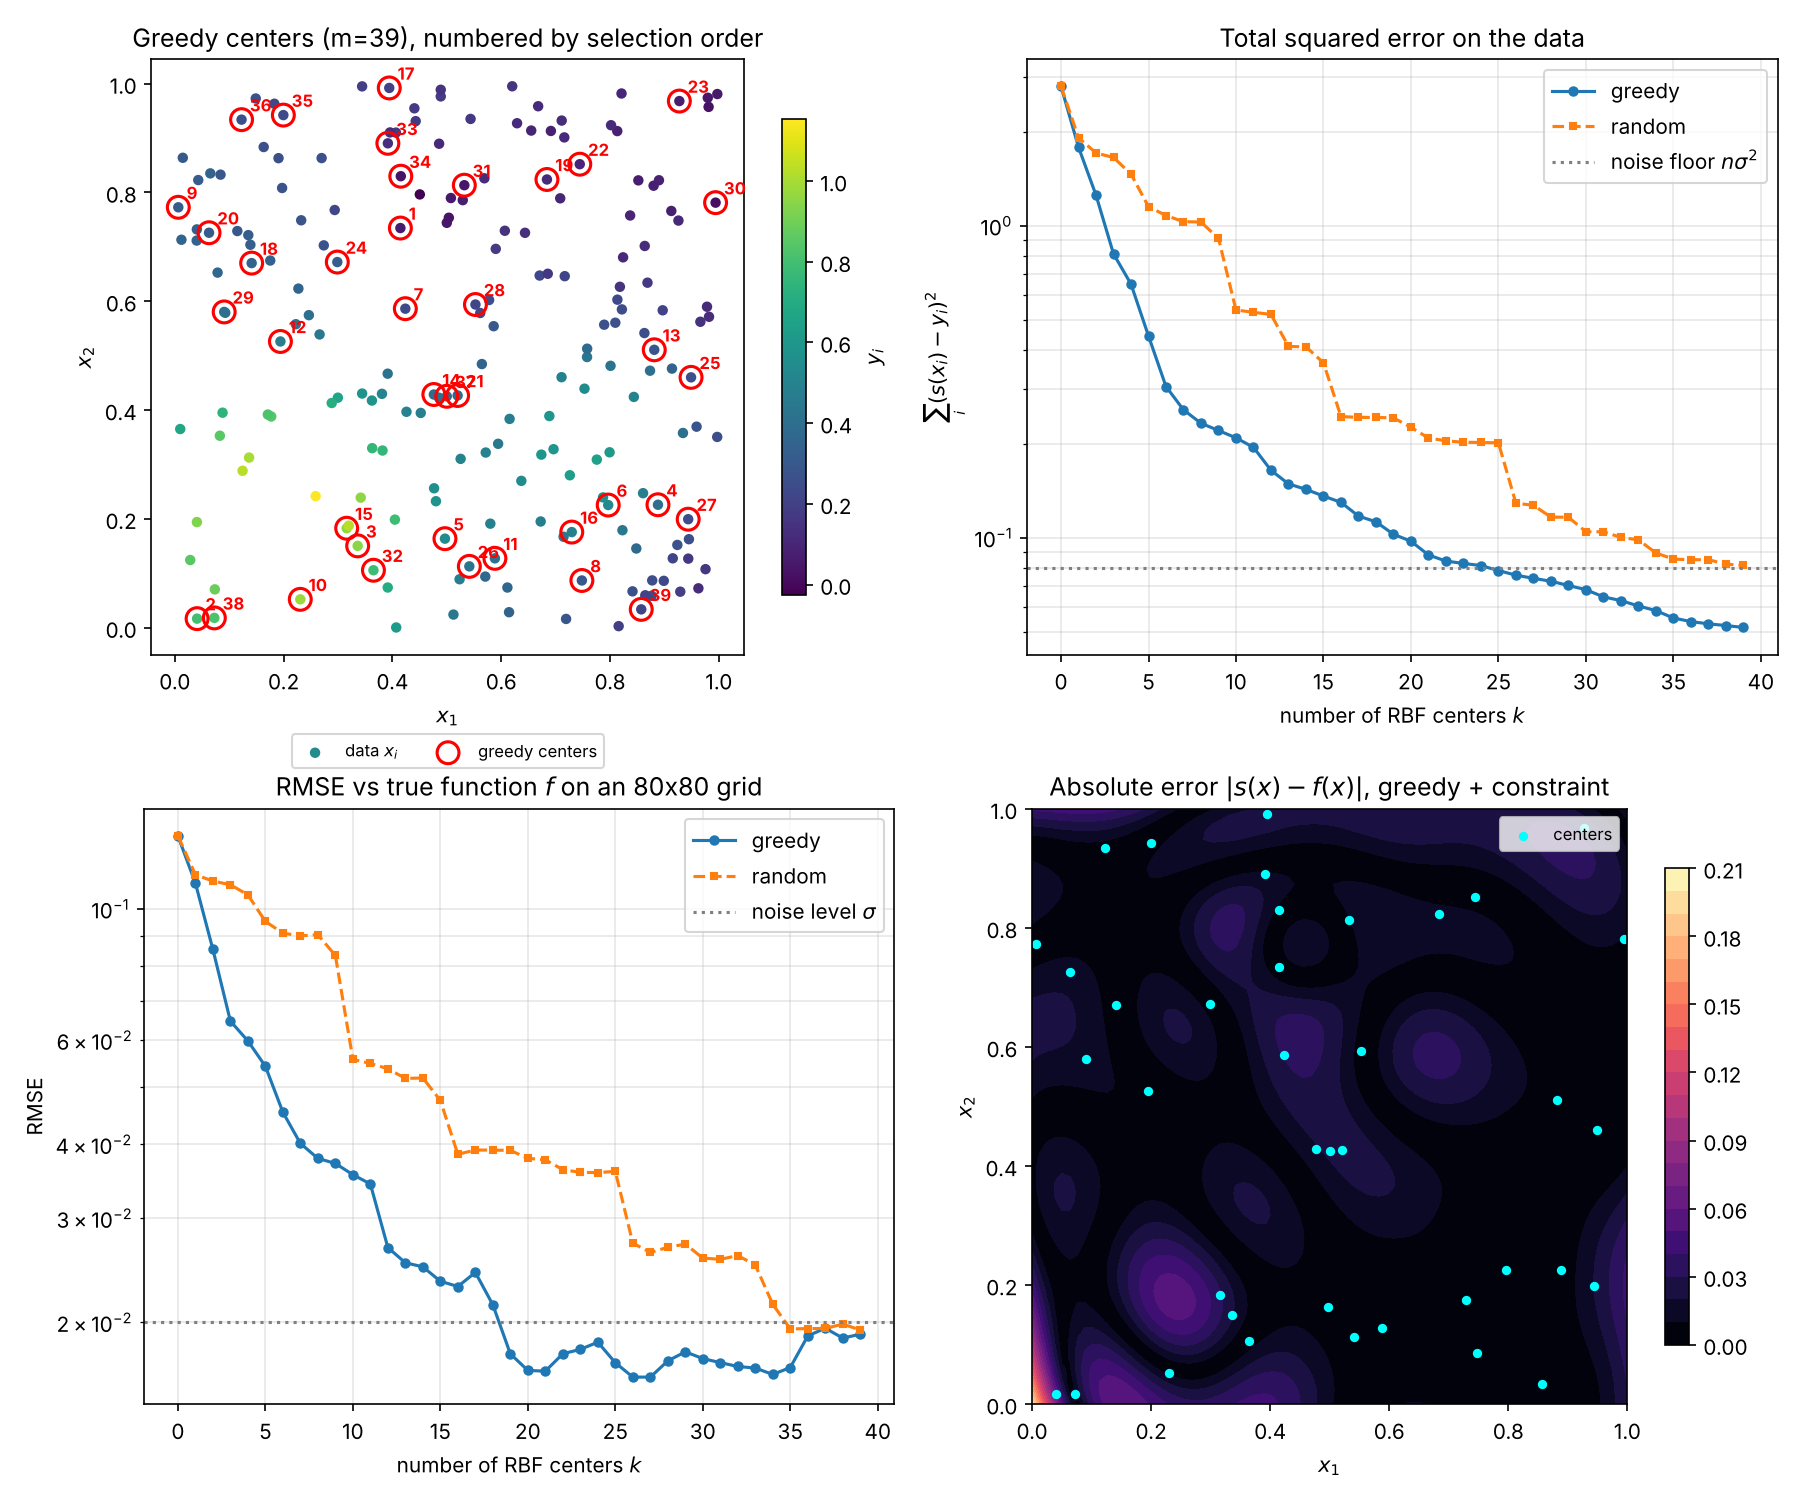
\includegraphics[width=\linewidth,height=0.80\textheight,keepaspectratio,trim=0 350 432 0,clip]{example02_results.png}
    \end{column}
    \begin{column}{0.43\textwidth}
      \begin{itemize}
        \item Red circles: the 39 greedy centers; the number is the order of selection.
        \item The first centers go to the main features of $f$ (peaks and valleys).
        \item Compare with the random centers of Example~1.
      \end{itemize}
    \end{column}
  \end{columns}
\end{frame}

\begin{frame}{Example 2: error on the data vs.\ number of centers}
  \begin{columns}[c]
    \begin{column}{0.55\textwidth}
      \centering
      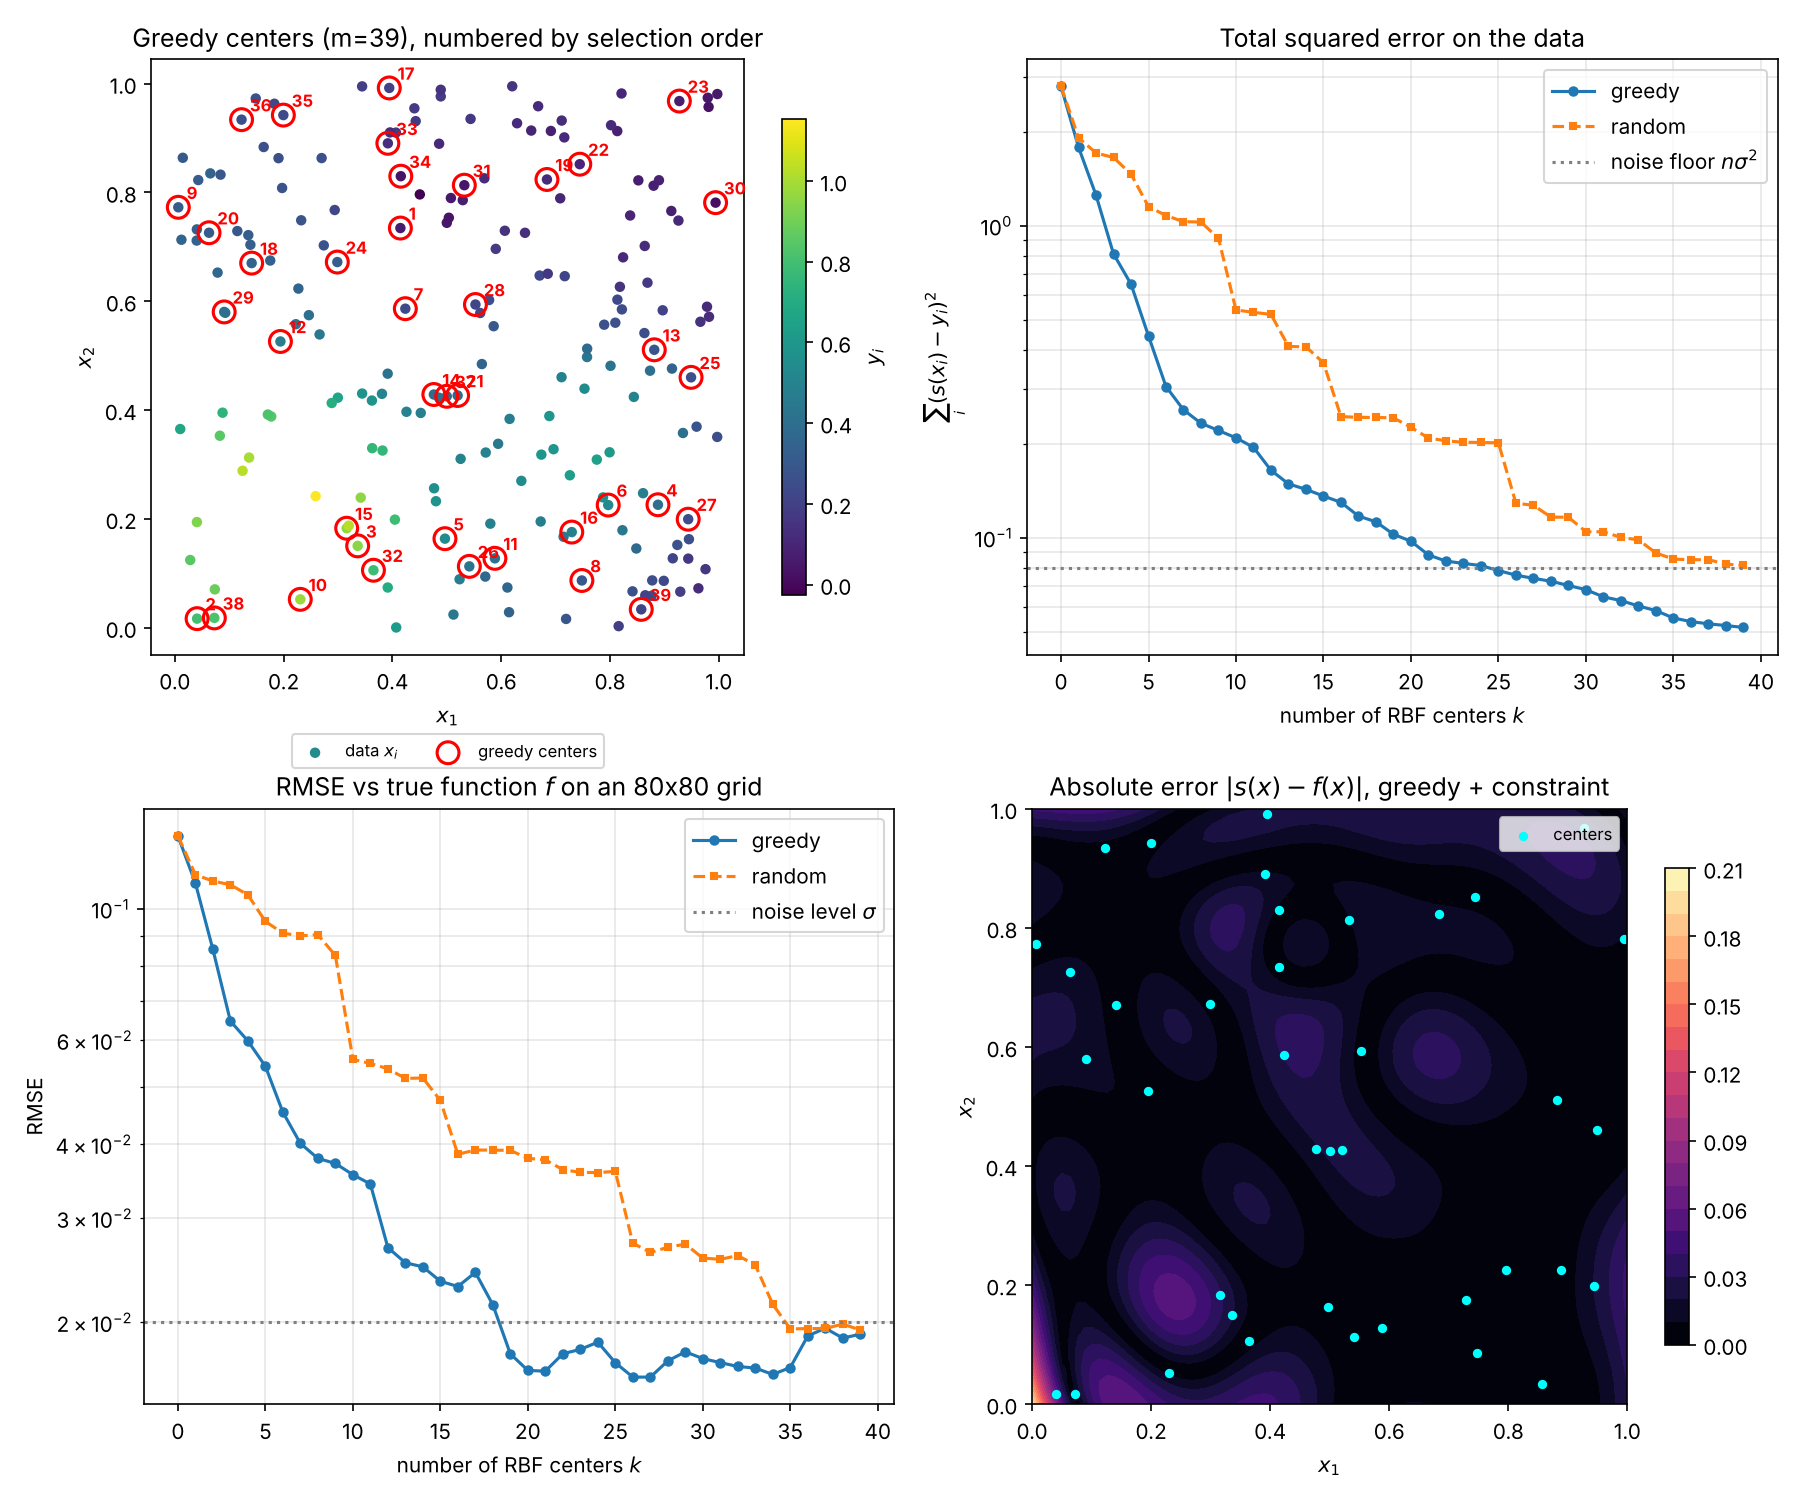
\includegraphics[width=\linewidth,height=0.80\textheight,keepaspectratio,trim=432 350 0 0,clip]{example02_results.png}
    \end{column}
    \begin{column}{0.43\textwidth}
      \begin{itemize}
        \item Total squared error on the data (log scale).
        \item Blue: greedy. Orange: random, one center at a time.
        \item Greedy decreases much faster.
        \item Dotted line: noise floor $n\sigma^2$. Greedy crosses it at $k\approx 25$.
      \end{itemize}
    \end{column}
  \end{columns}
\end{frame}

\begin{frame}{Example 2: true error vs.\ number of centers}
  \begin{columns}[c]
    \begin{column}{0.55\textwidth}
      \centering
      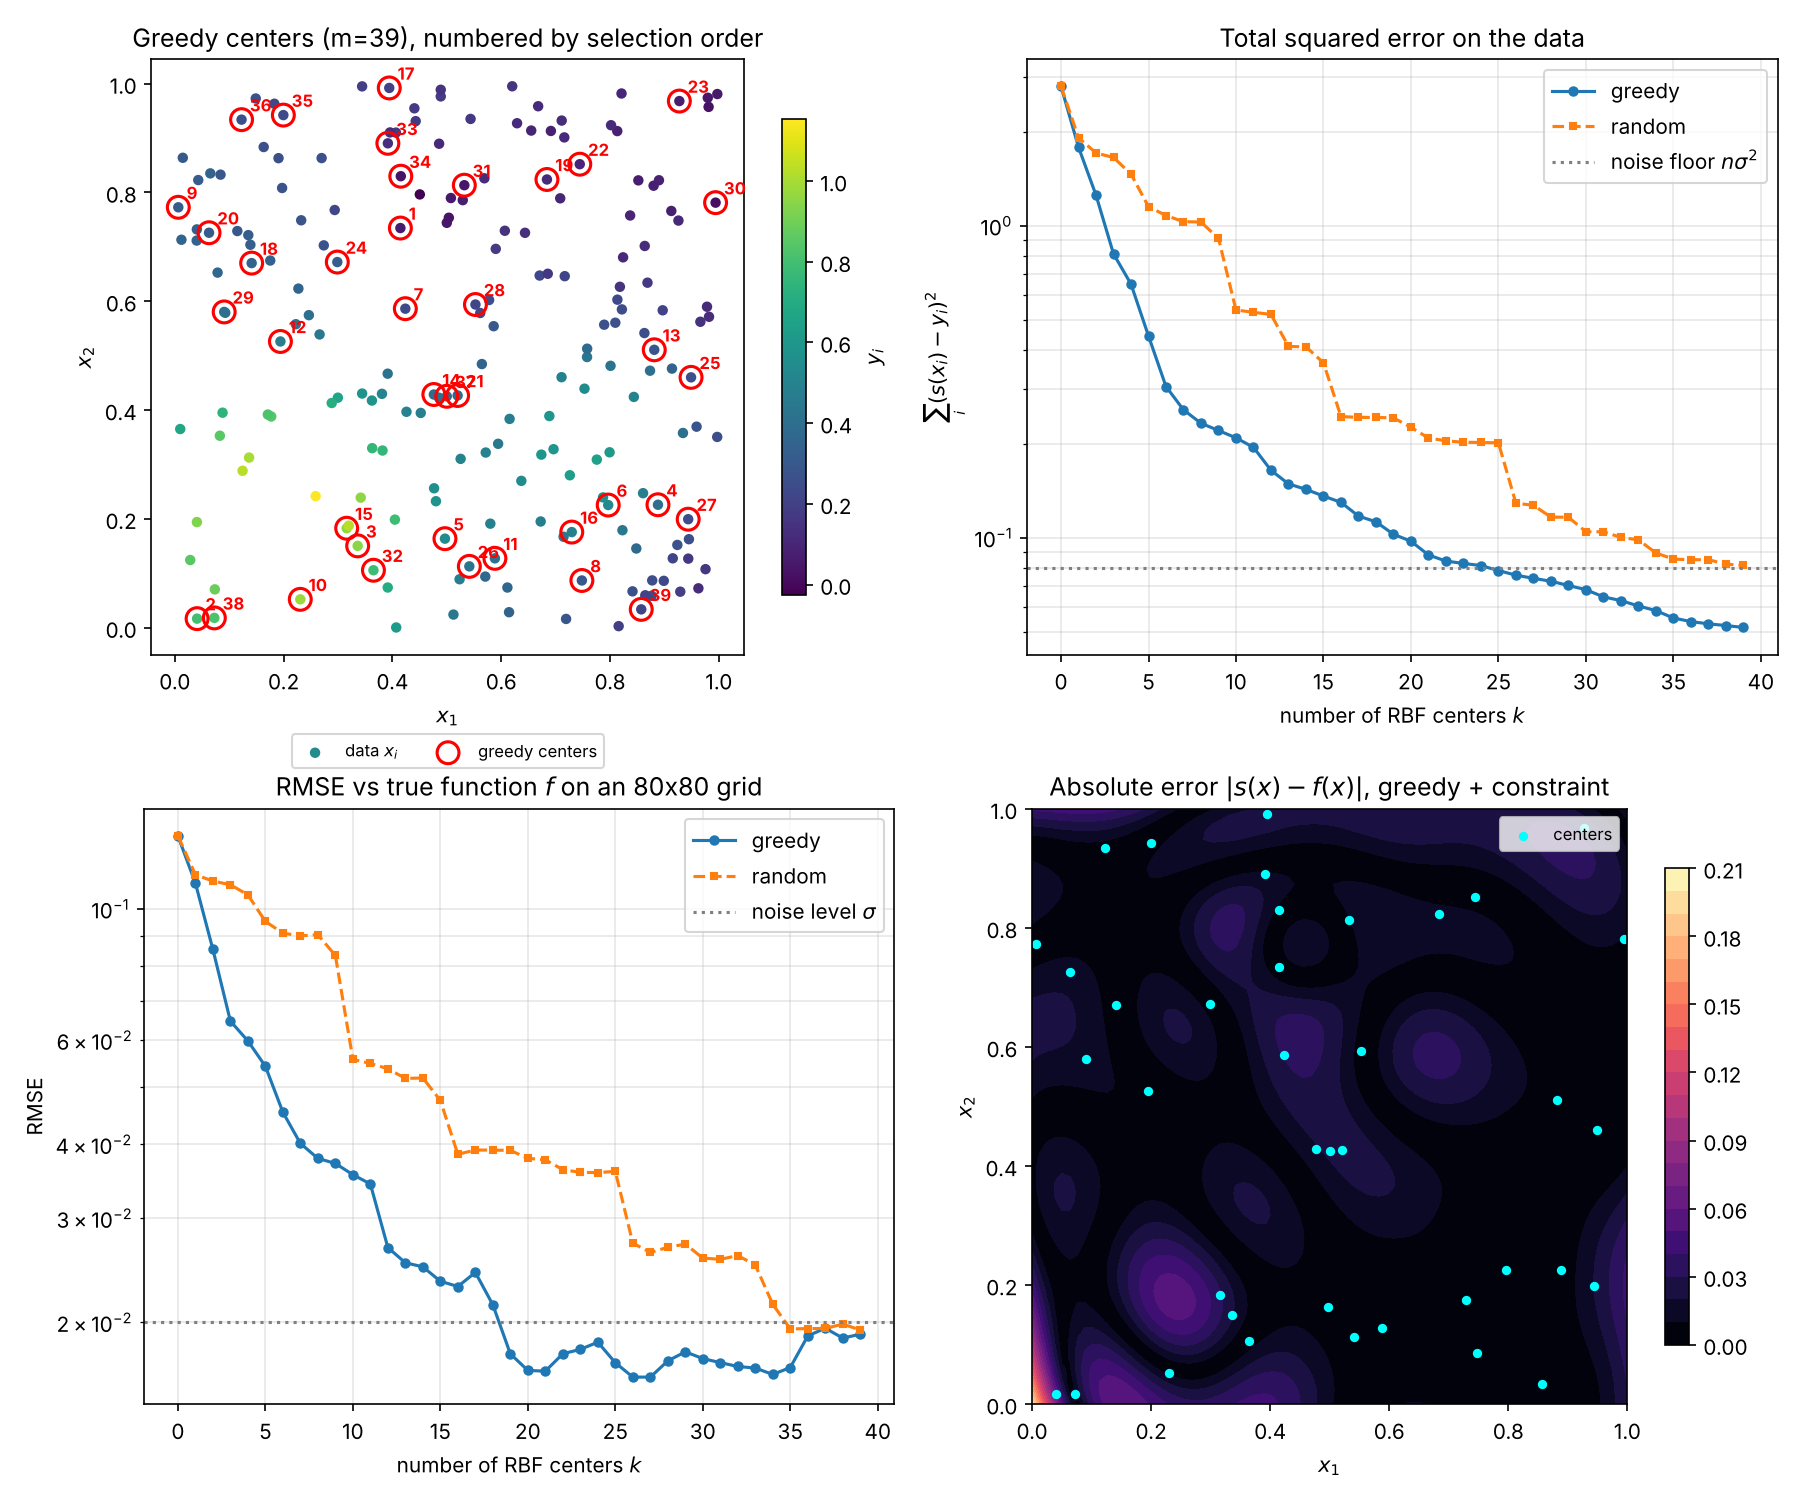
\includegraphics[width=\linewidth,height=0.80\textheight,keepaspectratio,trim=0 0 432 370,clip]{example02_results.png}
    \end{column}
    \begin{column}{0.43\textwidth}
      \begin{itemize}
        \item RMSE against the true $f$ on an $80\times80$ grid.
        \item Greedy reaches the noise level $\sigma$ with $\approx 20$ centers.
        \item After that it no longer improves: extra centers fit the noise.
        \item Possible only because we know $f$!
      \end{itemize}
    \end{column}
  \end{columns}
\end{frame}

\begin{frame}{Example 2: error map of the final model}
  \begin{columns}[c]
    \begin{column}{0.55\textwidth}
      \centering
      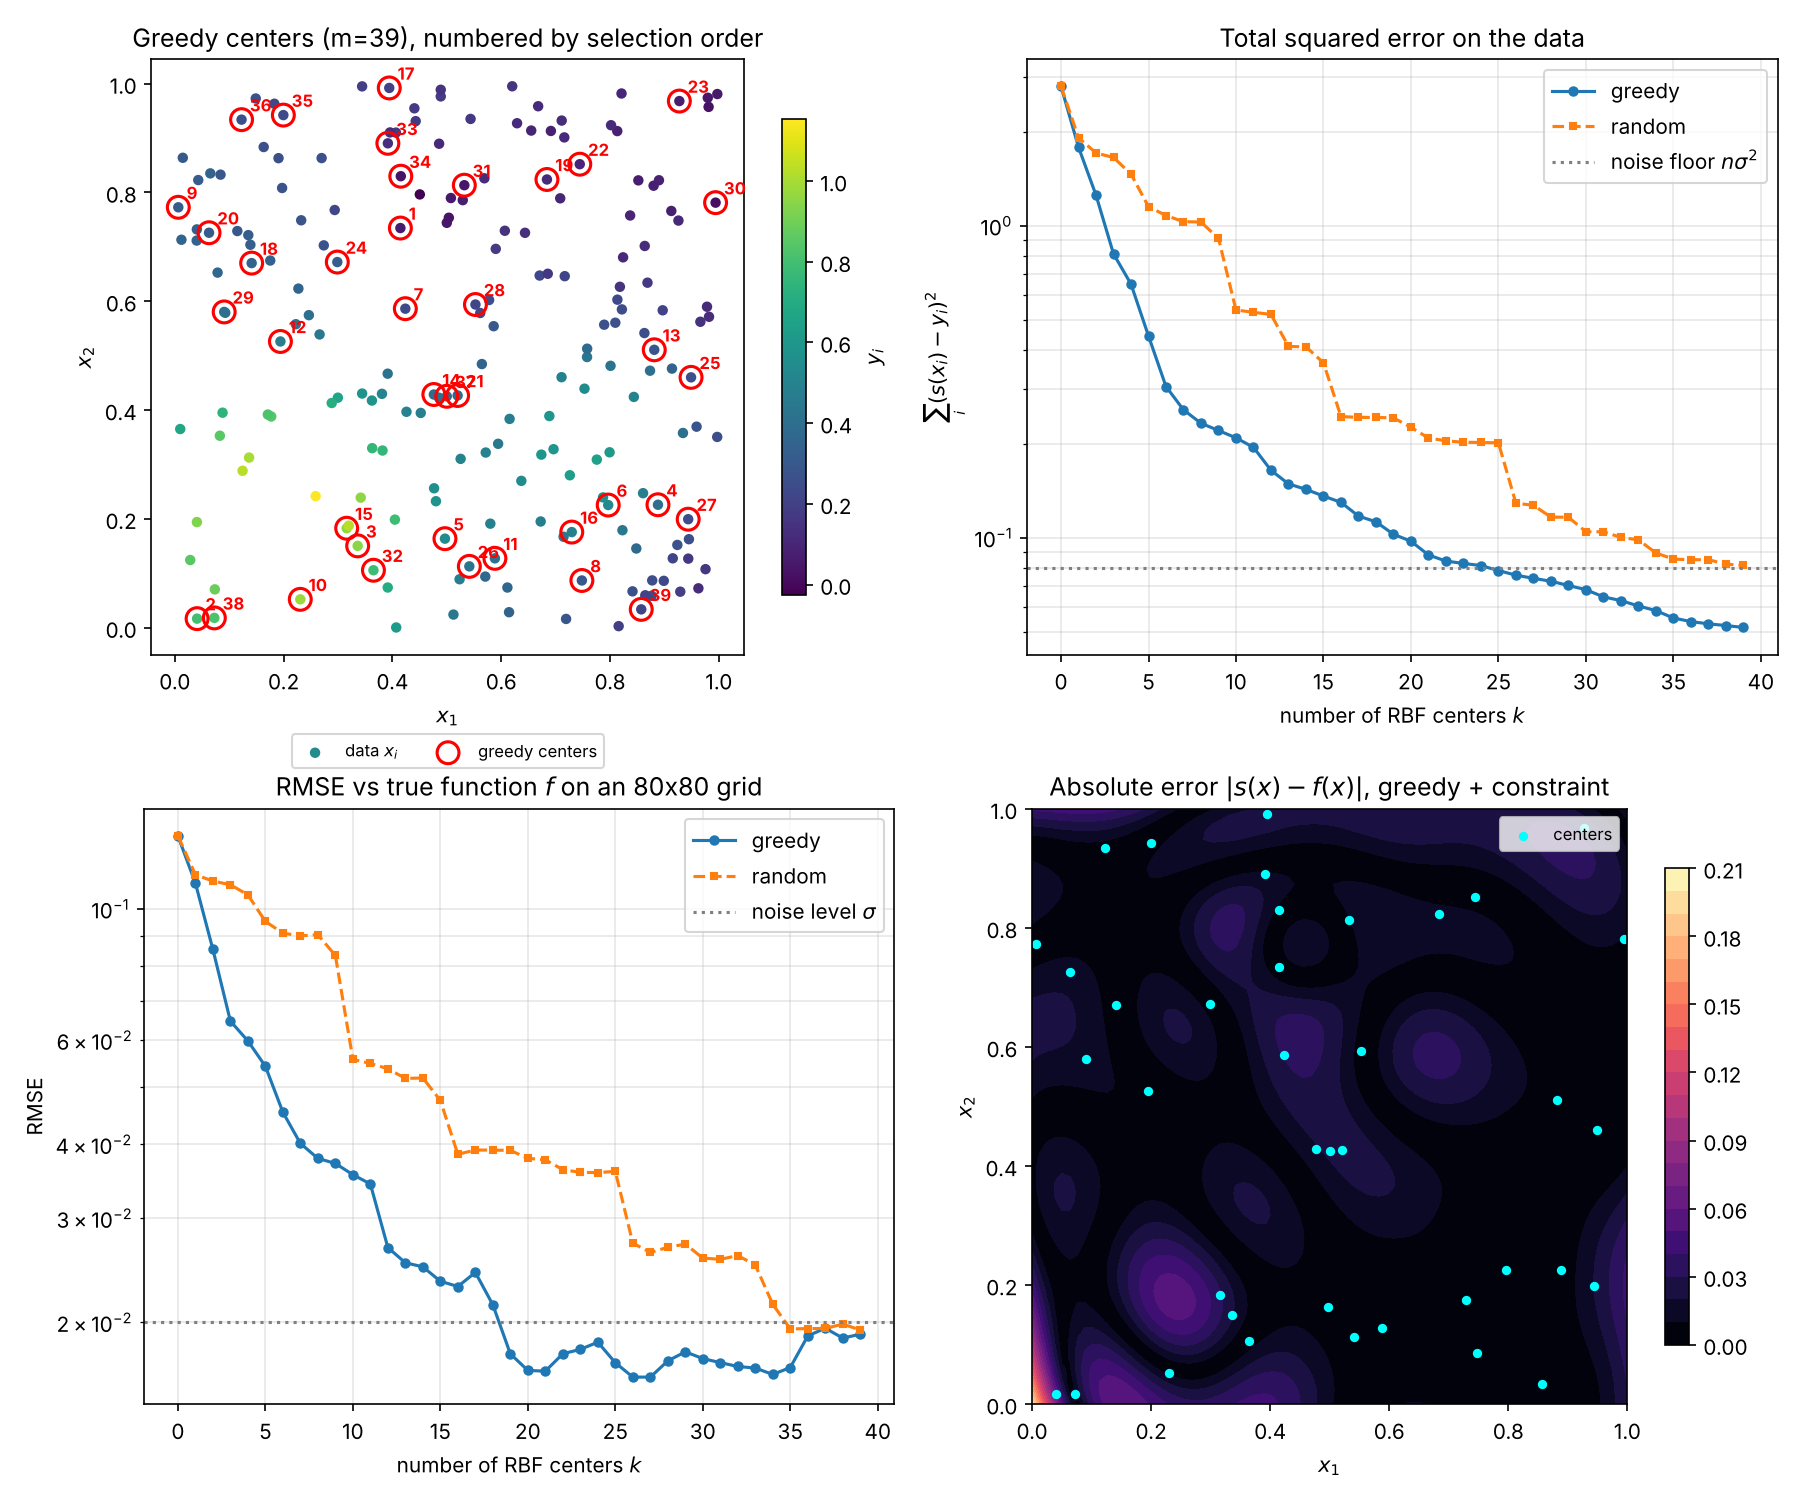
\includegraphics[width=\linewidth,height=0.80\textheight,keepaspectratio,trim=432 0 0 370,clip]{example02_results.png}
    \end{column}
    \begin{column}{0.43\textwidth}
      \begin{itemize}
        \item Final model: greedy centers + constraint (SLSQP).
        \item Lower RMSE than Example~1 ($0.018$ vs.\ $0.027$).
        \item But the \hl{maximum} error is larger ($\approx 0.21$), at the left edge near $(0,0)$, where the model extrapolates beyond the data.
        \item Greedy minimizes the \emph{squared} error on the data, not the worst-case error.
      \end{itemize}
    \end{column}
  \end{columns}
\end{frame}

\begin{frame}{Observation 1: greedy vs.\ random}
  \begin{itemize}
    \item ``Random'' = each new center is a random point not yet used
          (nested sets, same growth one center at a time). The first 30 are
          exactly the centers of Example~1.
    \item With greedy selection the error drops much faster:
  \end{itemize}
  \vspace{0.3em}
  \centering
  \begin{tabular}{lcc}
    \toprule
    To reach RMSE $\le 0.025$ vs.\ $f$ & Greedy & Random \\
    \midrule
    Number of centers needed & 13 & 33 \\
    \bottomrule
  \end{tabular}
  \vspace{0.5em}

  \raggedright
  \begin{itemize}
    \item The first greedy centers go where $f$ has its main features.
    \item The random curve is \hl{one realization}: another seed gives
          different steps. A fair comparison averages several random runs.
  \end{itemize}
\end{frame}

\begin{frame}{Observation 2: the error on the data always decreases}
  \begin{itemize}
    \item The SSE on the data decreases at every step: more terms
          \emph{always} fit the data better.
    \item The error against the true $f$ stops improving after
          $\approx 20$ centers and even grows slightly
          (minimum $0.016$ at $k\approx 26$, $0.019$ at $k=39$).
    \item After that point the model starts fitting the \hl{noise}:
          this is \hl{overfitting}.
  \end{itemize}
  \vspace{0.5em}
  \begin{alertblock}{Careful!}
    We can \emph{see} the overfitting only because we know $f$. In a real
    problem we only have the data, and the SSE on the data never warns us.
  \end{alertblock}
\end{frame}

\begin{frame}{Observation 3: detecting overfitting with the data only}
  \textbf{Discrepancy principle (Morozov):} do not fit the data more
  accurately than the noise in them.
  \[
    \text{stop when}\quad \textstyle\sum_i (s(\x_i)-y_i)^2 \;\le\; n\,\sigma^2
    \qquad (\text{here } n\sigma^2 = 0.08 \;\Rightarrow\; k \approx 25)
  \]
  \begin{itemize}
    \item Needs $\sigma$ (instrument precision, or an estimate).
    \item More precisely the target is $(n-p)\,\sigma^2$, with $p = k+6$
          fitted parameters.
  \end{itemize}
  \textbf{Validation:} measure the error on points \emph{not used} in the fit.
  \begin{itemize}
    \item Hold-out set (e.g.\ 20\% of the data) or $k$-fold cross-validation.
    \item Leave-one-out (LOOCV), cheap for linear least squares:
          \[
            e_i^{\text{LOO}} = \frac{r_i}{1 - h_{ii}}, \qquad
            H = A(A^TA)^{-1}A^T
          \]
  \end{itemize}
\end{frame}

\begin{frame}{Observation 4: what greedy does and does not guarantee}
  \begin{itemize}
    \item At each step, the chosen center is the \hl{best possible} given
          the centers already selected (all candidates are tried).
    \item But greedy never revisits earlier choices: the final set is
          \hl{not} necessarily the best set of 39 centers.
    \item The global optimum would require trying all subsets:
          \[
            \binom{200}{39} \approx 5\times 10^{41}\ \text{combinations}
          \]
    \item Greedy does not penalize centers that are very close together
          (e.g.\ centers 14 and 21 near $(0.5, 0.43)$): nearly equal columns
          in $A$ $\Rightarrow$ worse conditioning.
    \item Efficient versions update a QR factorization instead of refitting
          from scratch (orthogonal matching pursuit).
  \end{itemize}
\end{frame}

% =====================================================================
\section{Example 3: stochastic gradient methods}
% =====================================================================

\begin{frame}{How Machine Learning would solve this problem}
  In Machine Learning (ML) the usual tools are different:
  \begin{itemize}
    \item \hl{No constraints}: everything goes into one loss function.
    \item \hl{Stochastic gradient} methods: cheap steps that use only a small
          random part of the data. They scale to millions of data points.
    \item Speed is often preferred over an accurate minimization.
  \end{itemize}
  \vspace{0.5em}
  \textbf{Example 3} solves exactly the problem of Example 1 (same data,
  same 30 random centers, $\varepsilon=3$, quadratic polynomial) in that way:
  \begin{enumerate}[(a)]
    \item the orthogonality conditions become extra equations of the system;
    \item the loss is minimized with SGD, SGD with momentum and Adam.
  \end{enumerate}
  \vspace{0.5em}
  \begin{alertblock}{Question}
    How close do these methods get to the true minimum?
  \end{alertblock}
\end{frame}

\begin{frame}{(a) The orthogonality conditions as extra equations}
  Append the 6 conditions $P_c^T\bm{a}=\bm{0}$, multiplied by a weight
  $\lambda$, below the collocation system:
  \[
    \underbrace{\begin{bmatrix} \Phi & P \\ \lambda P_c^T & 0 \end{bmatrix}}_{A_{\text{aug}}\;((n+6)\times p)}
    \begin{bmatrix} \bm{a} \\ \bm{b} \end{bmatrix}
    \approx
    \underbrace{\begin{bmatrix} \bm{y} \\ \bm{0} \end{bmatrix}}_{\bm{y}_{\text{aug}}}
  \]
  One unconstrained least-squares problem:
  \[
    L(\bm{w}) = \tfrac12 \lVert A_{\text{aug}}\bm{w} - \bm{y}_{\text{aug}} \rVert^2
    = \tfrac12 \sum_{i=1}^{n} \big(s(\x_i) - y_i\big)^2
      + \tfrac12 \lambda^2 \lVert P_c^T \bm{a} \rVert^2
  \]
  \begin{itemize}
    \item The constraint is now satisfied only \emph{approximately}: it
          competes with the data. A larger $\lambda$ enforces it more.
    \item We use $\lambda = 1$. The exact minimum of $L$ is computed with
          \texttt{lstsq} as a reference.
  \end{itemize}
\end{frame}

\begin{frame}{Gradient descent: walking downhill}
  \begin{columns}[c]
    \begin{column}{0.55\textwidth}
      $L(\bm{w})$ is a quadratic function: its graph is a \hl{valley}
      (a paraboloid). The minimum is at the bottom.
      \vspace{0.5em}

      \textbf{Gradient descent:} take steps in the downhill direction
      \[
        \bm{w} \leftarrow \bm{w} - \alpha\, \nabla L(\bm{w})
      \]
      $\alpha$ is the step size (\emph{learning rate}).
      \vspace{0.5em}

      For our problem the gradient is
      \[
        \nabla L = A^T(A\bm{w} - \bm{y})
        = \sum_{i=1}^{n} \bm{a}_i \big(\bm{a}_i^T \bm{w} - y_i\big)
      \]
      where $\bm{a}_i^T$ is row $i$ of $A$.
      \hl{The gradient is a sum over the data.}
    \end{column}
    \begin{column}{0.42\textwidth}
      \centering
      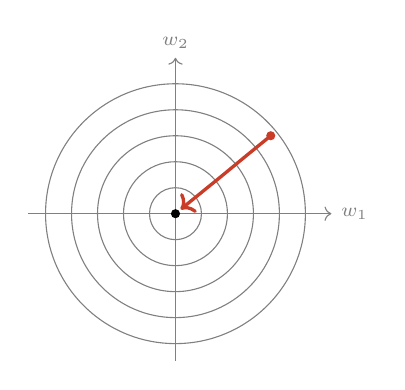
\begin{tikzpicture}[scale=1.1]
        \foreach \r in {0.3,0.6,0.9,1.2,1.5} \draw[gray] (0,0) circle (\r);
        \draw[->,gray] (-1.7,0) -- (1.8,0) node[right] {\scriptsize $w_1$};
        \draw[->,gray] (0,-1.7) -- (0,1.8) node[above] {\scriptsize $w_2$};
        \draw[accent,very thick,->] (1.1,0.9) -- (0.77,0.63) -- (0.54,0.44) -- (0.38,0.31) -- (0.06,0.05);
        \fill[accent] (1.1,0.9) circle (1.5pt);
        \fill (0,0) circle (1.5pt);
      \end{tikzpicture}

      {\scriptsize A round valley: each step points to the minimum.}
    \end{column}
  \end{columns}
\end{frame}

\begin{frame}{Stochastic gradient: estimate the sum with a sample}
  If $n$ is huge, computing the full sum at every step is expensive.
  \textbf{Idea:} estimate it from a small random sample, like an opinion
  poll estimates the opinion of a whole country.
  \vspace{0.3em}
  \begin{itemize}
    \item Choose a random \hl{mini-batch} $B$ of data indices, e.g.\ $|B| = 20$.
    \item Estimate the gradient with those rows only:
          \[
            \bm{g}_B = \frac{n}{|B|} \sum_{i \in B} \bm{a}_i \big(\bm{a}_i^T \bm{w} - y_i\big)
            \qquad (\text{the factor } n/|B| \text{ turns the sample average into a full sum})
          \]
    \item Step: $\bm{w} \leftarrow \bm{w} - \alpha\, \bm{g}_B$.
          Cost per step: $|B|$ rows, \hl{independent of $n$}.
    \item \textbf{Epoch:} one pass over the data ($n/|B| = 10$ steps here).
          Each epoch the data are shuffled.
    \item The 6 constraint rows are always included in $\bm{g}_B$.
  \end{itemize}
  \vspace{0.3em}
  \small The estimate is \emph{noisy}: each step points only roughly downhill.
\end{frame}

\begin{frame}{Accelerated variants: momentum and Adam}
  \textbf{SGD with momentum} (``heavy ball''): average the recent gradients
  \[
    \bm{m} \leftarrow \beta\,\bm{m} + \bm{g}_B, \qquad
    \bm{w} \leftarrow \bm{w} - \alpha\,\bm{m}, \qquad \beta = 0.9
  \]
  The noise partly cancels, and the method keeps moving along consistent
  directions.
  \vspace{0.5em}

  \textbf{Adam} (the standard in ML): a separate step size for every
  coordinate
  \[
    \bm{m} \leftarrow 0.9\,\bm{m} + 0.1\,\bm{g}_B, \qquad
    \bm{s} \leftarrow 0.999\,\bm{s} + 0.001\,\bm{g}_B^2, \qquad
    w_j \leftarrow w_j - \alpha\, \frac{m_j}{\sqrt{s_j} + 10^{-8}}
  \]
  (with a small bias correction of $\bm{m}$ and $\bm{s}$ in the first steps).
  Coordinates with large gradients get smaller steps.
  \vspace{0.5em}

  All three use only \hl{gradients}: they are \hl{first-order} methods.
\end{frame}

\begin{frame}{Preprocessing the columns of $A$}
  ML practitioners always normalize the features (the columns of $A$).
  We try three options, each a change of variables $\bm{w} = T\bm{v}$
  (we optimize $\bm{v}$, then recover $\bm{w}$):
  \vspace{0.3em}
  \begin{center}
  \begin{tabular}{llc}
    \toprule
    Option & What it does & $\operatorname{cond}(A_{\text{aug}}T)$ \\
    \midrule
    raw & nothing & $2.2\times10^{6}$ \\
    scaled & each column divided by its norm & $2.5\times10^{6}$ \\
    standardized & RBF columns: mean 0, standard deviation 1 & $5.1\times10^{5}$ \\
    \bottomrule
  \end{tabular}
  \end{center}
  \begin{itemize}
    \item Scaling does \hl{not} help: the columns already have similar sizes.
          The problem is that MQ columns are \hl{almost collinear}.
    \item Standardizing removes their common part (the mean, absorbed by the
          constant polynomial term) and improves the conditioning
          $\approx 4$ times.
  \end{itemize}
\end{frame}

\begin{frame}{Example 3: results after 100\,000 iterations}
  \centering\small
  \begin{tabular}{lcccc}
    \toprule
    Solution & $L/L_{\min}$ & RMSE vs.\ $f$ & $\lVert\bm{w}\rVert$ & time \\
    \midrule
    \texttt{lstsq} (exact minimum) & 1.00 & 0.027 & 608 & 0.001\,s \\
    Example 1 (SLSQP, exact constraint) & 1.01 & 0.027 & 704 & 0.02\,s \\
    \midrule
    SGD, raw & 11.8 & 0.097 & 1.2 & 1.2\,s \\
    SGD, scaled & 11.4 & 0.095 & 1.8 & 1.2\,s \\
    SGD + momentum, standardized & 4.4 & 0.061 & 4.4 & 1.2\,s \\
    Adam, raw & 8.5 & 0.081 & 4.9 & 1.9\,s \\
    \hl{Adam, standardized} (best) & \hl{3.3} & \hl{0.049} & 11.5 & 2.1\,s \\
    \bottomrule
  \end{tabular}
  \vspace{0.8em}

  \raggedright
  \begin{itemize}
    \item \hl{No} stochastic method reaches the minimum. The best one ends
          3 times above it, with almost twice the true error.
    \item On this small problem the exact solver is also much faster.
  \end{itemize}
\end{frame}

\begin{frame}{Example 3: the loss during training}
  \begin{columns}[c]
    \begin{column}{0.56\textwidth}
      \centering
      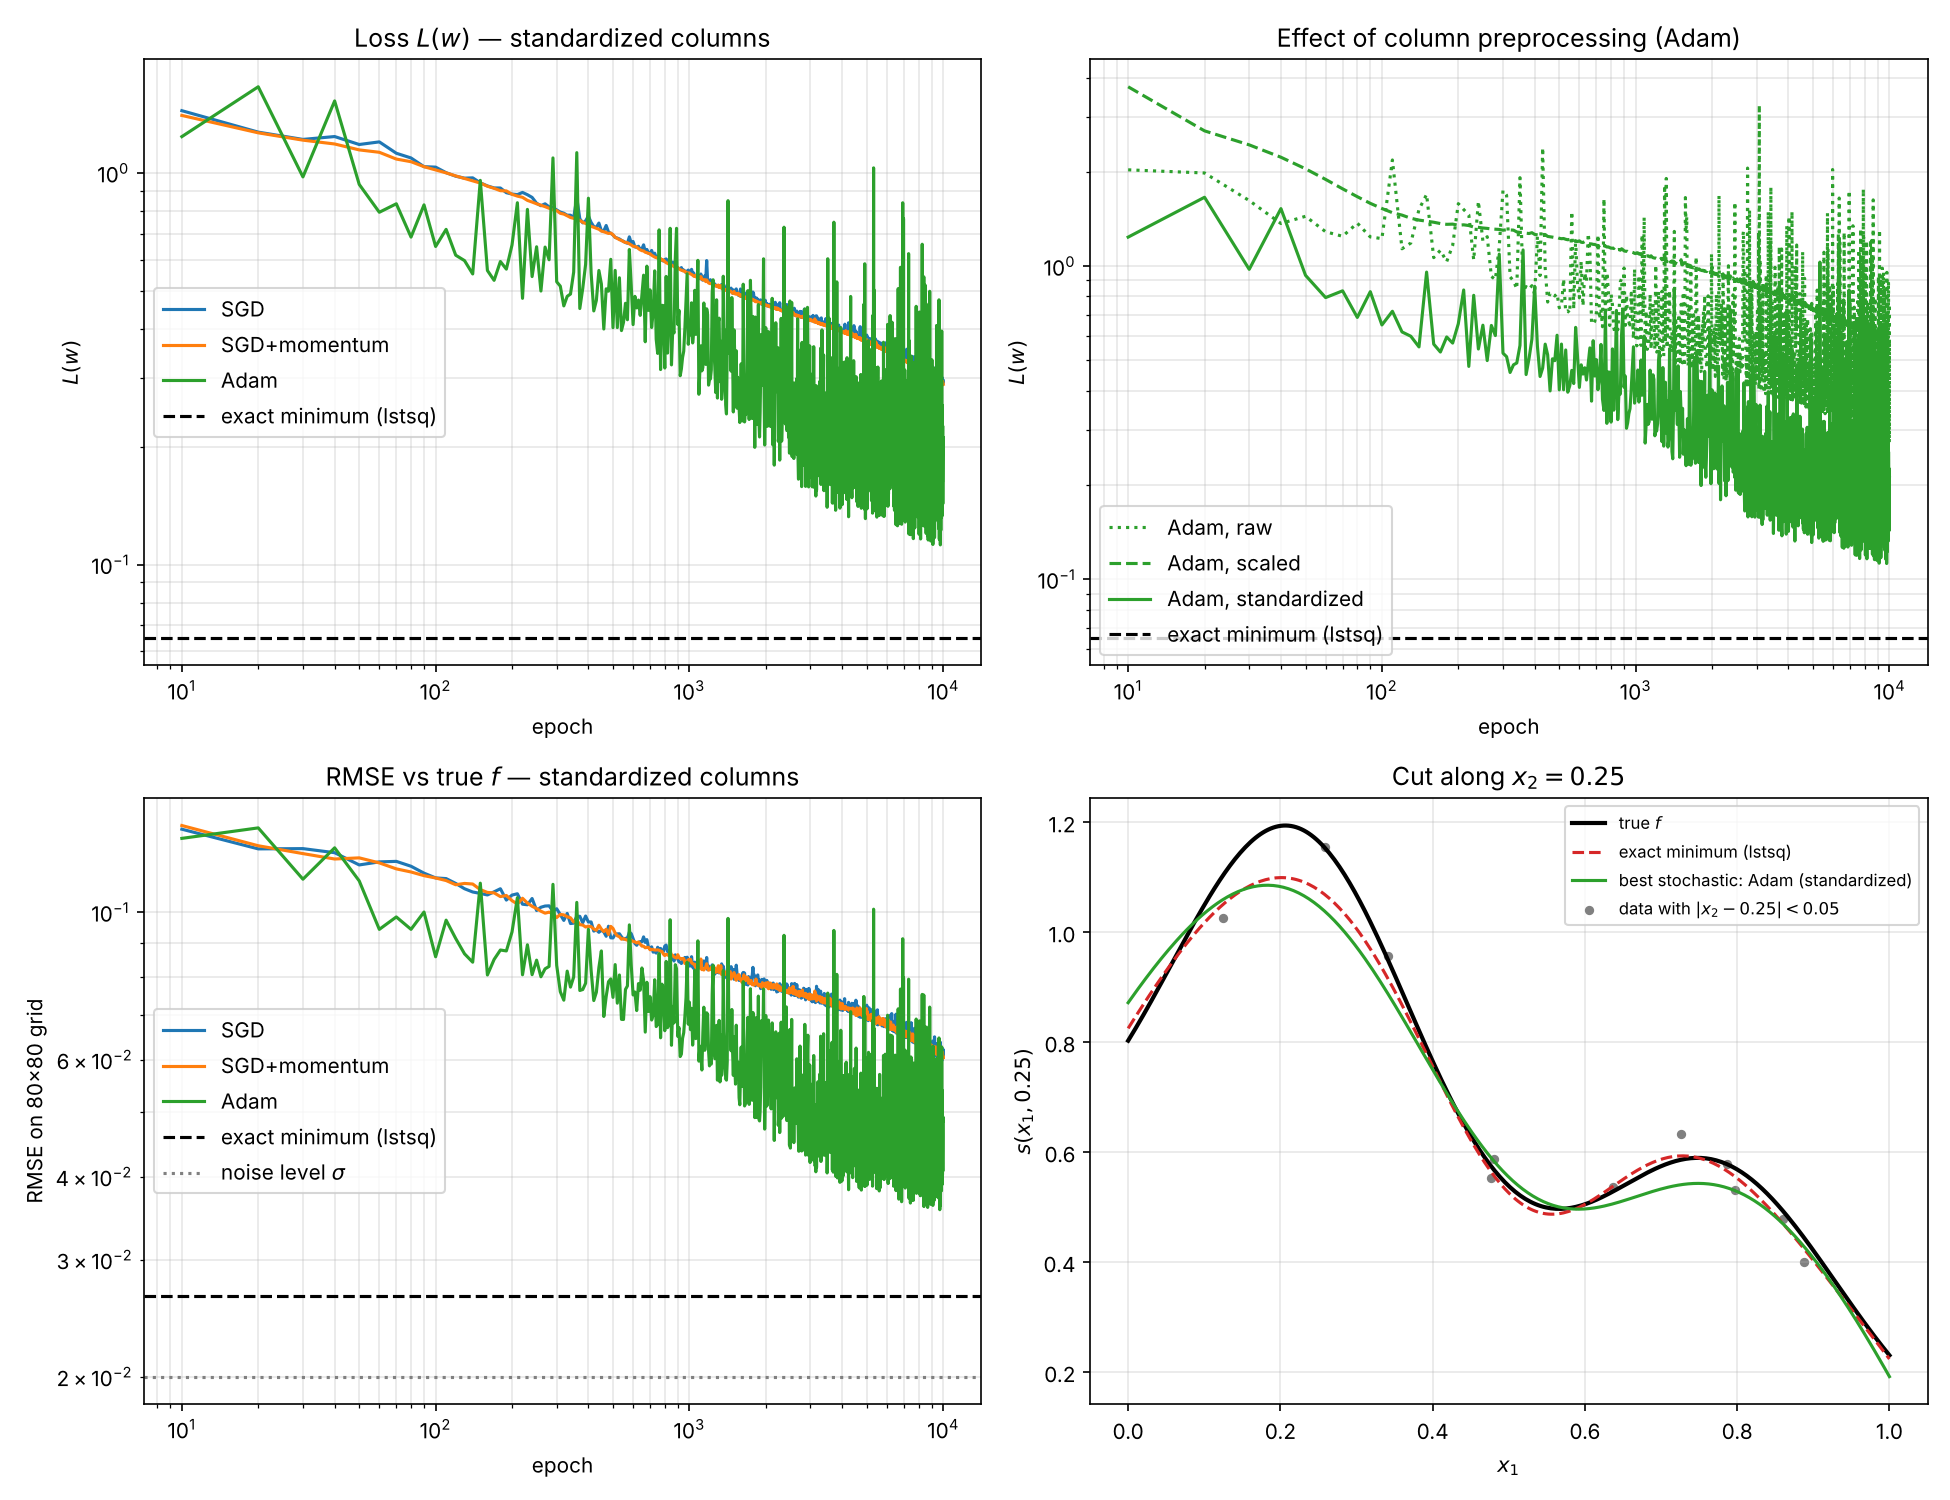
\includegraphics[width=\linewidth,height=0.80\textheight,keepaspectratio,trim=0 359 458 0,clip]{example03_results.png}
    \end{column}
    \begin{column}{0.42\textwidth}
      \begin{itemize}
        \item Loss $L(\bm{w})$ vs.\ epochs, standardized columns (log scales).
        \item Dashed line: the exact minimum.
        \item SGD and momentum: slow, steady decrease.
        \item Adam: faster at first, but it \hl{oscillates} (constant step size).
        \item After 10\,000 epochs all of them are still far from the minimum.
      \end{itemize}
    \end{column}
  \end{columns}
\end{frame}

\begin{frame}{Example 3: what the student sees}
  \begin{columns}[c]
    \begin{column}{0.56\textwidth}
      \centering
      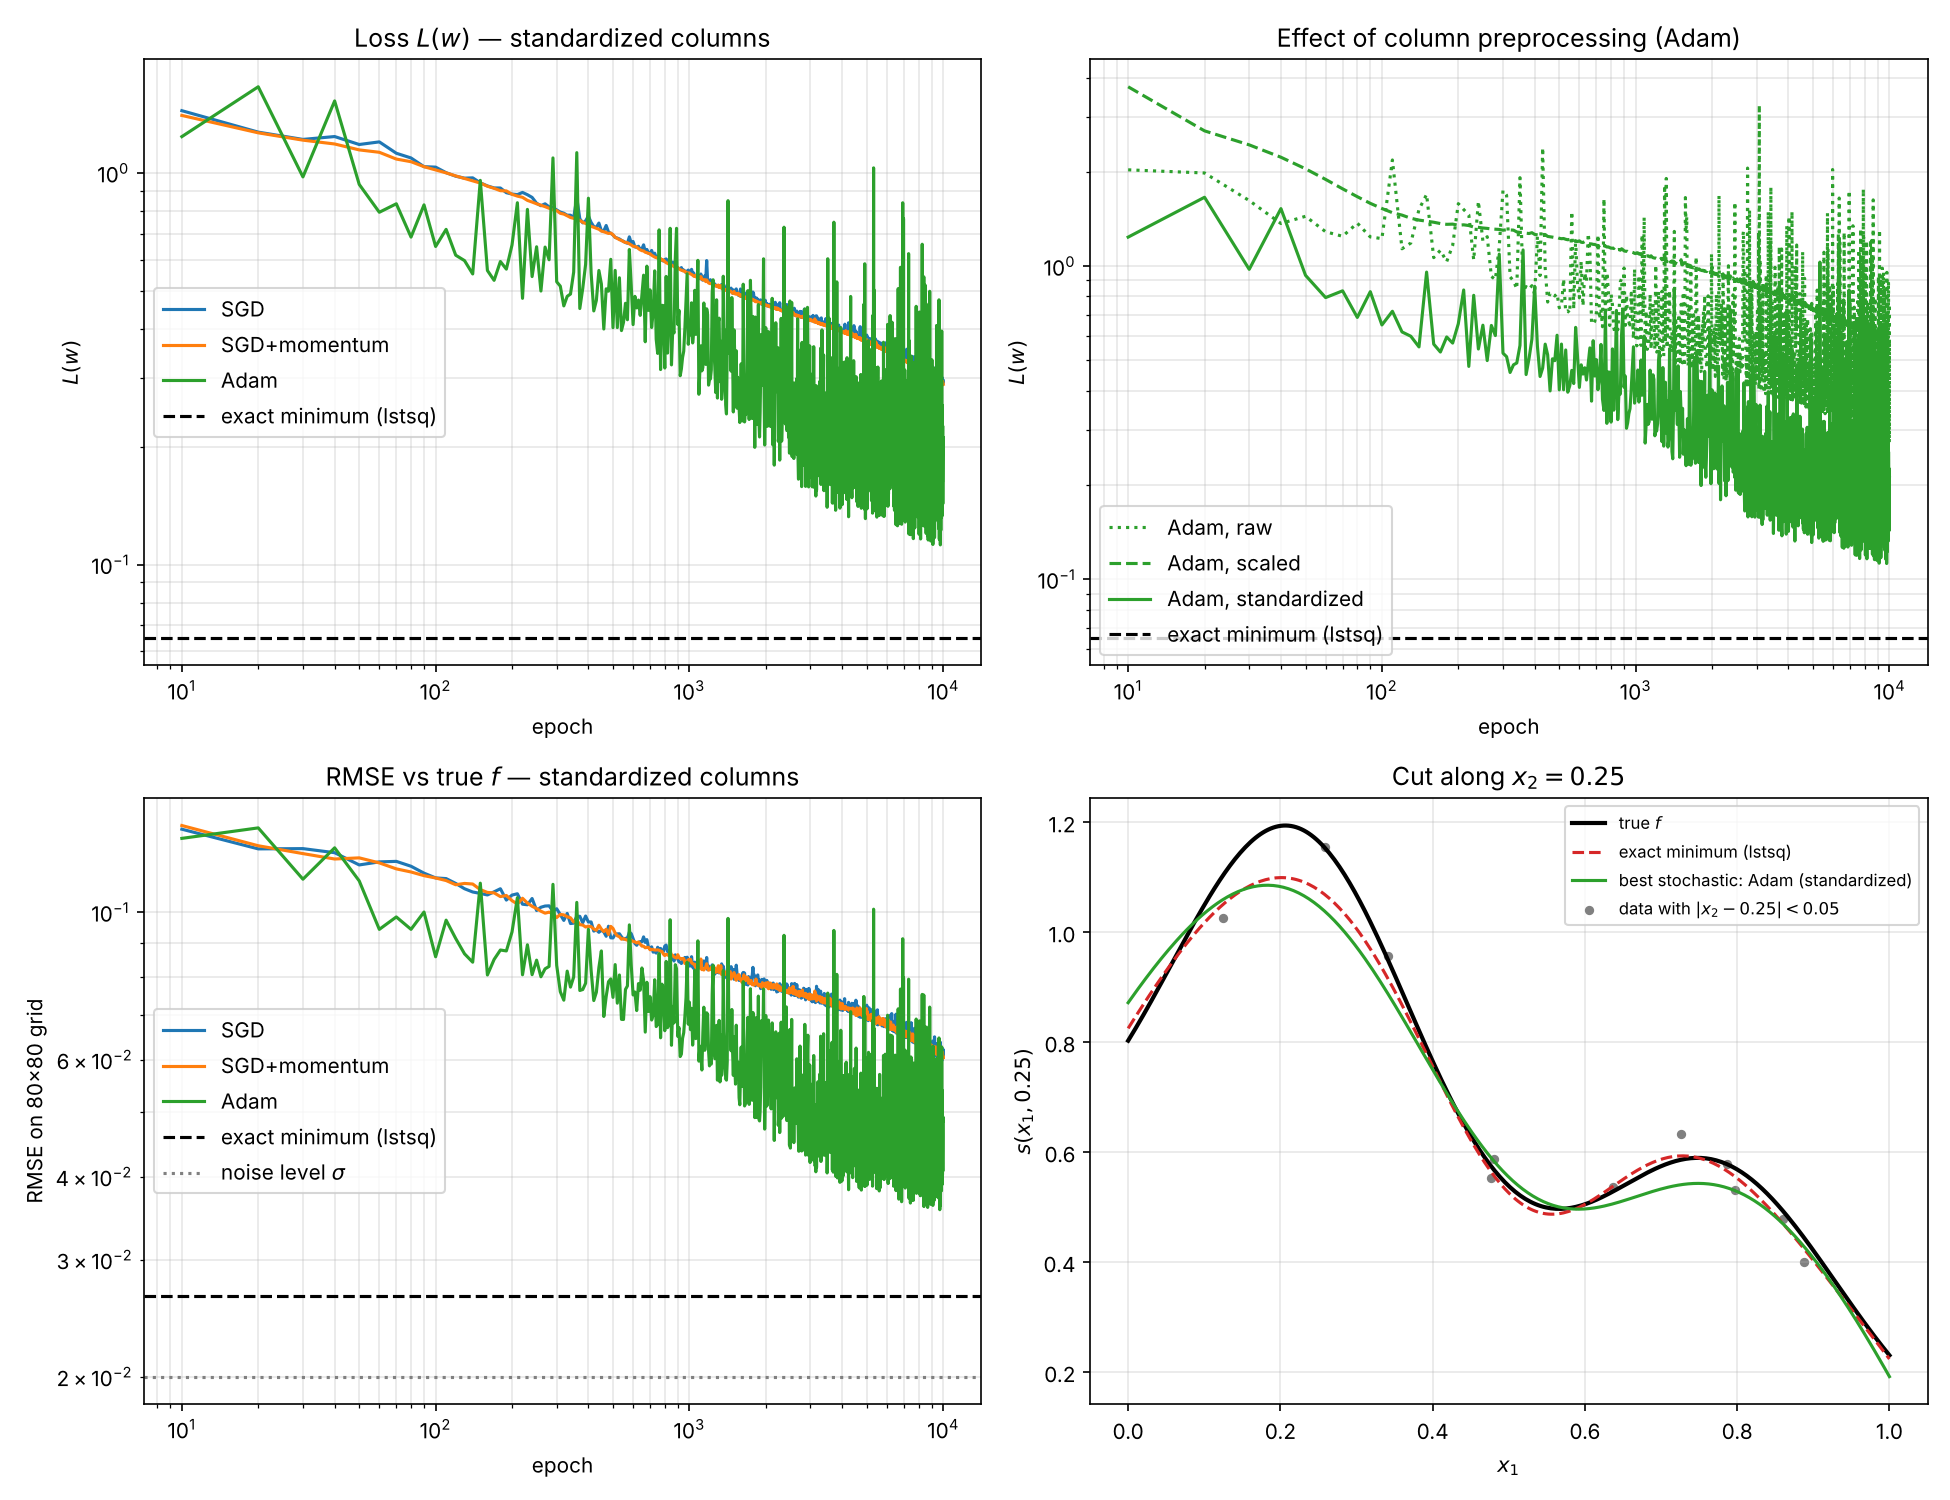
\includegraphics[width=\linewidth,height=0.80\textheight,keepaspectratio,trim=478 0 0 361,clip]{example03_results.png}
    \end{column}
    \begin{column}{0.42\textwidth}
      \begin{itemize}
        \item Cut of the models along $x_2 = 0.25$.
        \item Red dashed: exact minimum. Green: best stochastic model (Adam).
        \item The difference is visible: Adam misses the peaks.
        \item A poor minimization gives a poorer approximation.
      \end{itemize}
    \end{column}
  \end{columns}
\end{frame}

\begin{frame}{Why do gradient methods fail here?}
  \begin{columns}[c]
    \begin{column}{0.58\textwidth}
      Our valley is \hl{extremely elongated}. A 2D example:
      \[
        L = \tfrac12\big(1000\,w_1^2 + w_2^2\big)
      \]
      \begin{itemize}
        \item Direction $w_1$ is steep: a step $\alpha > 2/1000$ bounces from
              wall to wall and diverges. So $\alpha \approx 0.001$.
        \item Direction $w_2$ is almost flat: with $\alpha=0.001$ each step
              advances only $0.1\%$ of the remaining distance.
      \end{itemize}
      \vspace{0.3em}
      In our problem the ratio is not 1000 but
      $\kappa = \operatorname{cond}(A^TA) \approx 10^{13}$.
    \end{column}
    \begin{column}{0.40\textwidth}
      \centering
      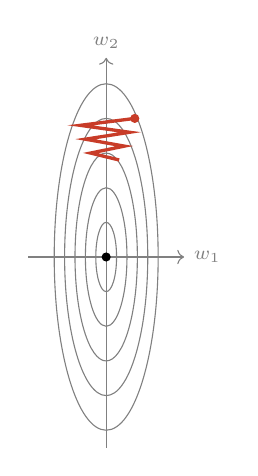
\begin{tikzpicture}[scale=1.1]
        \foreach \r in {0.4,0.8,1.2,1.6,2.0} \draw[gray] (0,0) ellipse ({0.3*\r} and {\r});
        \draw[->,gray] (-0.9,0) -- (0.9,0) node[right] {\scriptsize $w_1$};
        \draw[->,gray] (0,-2.2) -- (0,2.3) node[above] {\scriptsize $w_2$};
        \draw[accent,very thick] (0.33,1.6) -- (-0.3,1.52) -- (0.27,1.44) -- (-0.24,1.36) -- (0.21,1.28) -- (-0.18,1.2) -- (0.15,1.12);
        \fill[accent] (0.33,1.6) circle (1.5pt);
        \fill (0,0) circle (1.5pt);
      \end{tikzpicture}

      {\scriptsize Zig-zag across the valley, slow progress along it.}
    \end{column}
  \end{columns}
\end{frame}

\begin{frame}{This is a theorem, not a tuning problem}
  \begin{block}{Lower bound for first-order methods (Nesterov)}
    For quadratic functions, no method that only combines gradients can
    converge, in the worst case, faster than about
    \[
      \sqrt{\kappa}\;\log(1/\text{tol}) \quad \text{iterations.}
    \]
  \end{block}
  \begin{itemize}
    \item Here $\sqrt{\kappa} \approx 3\times10^{6}$. Momentum and Adam improve
          the constant, but cannot beat the bound.
    \item The exact solution has large coefficients that cancel each other
          ($\lVert\bm{w}^\ast\rVert \approx 600$). They live in the
          \hl{flat directions} of the valley, which gradient steps starting
          from $\bm{w}=\bm{0}$ explore extremely slowly
          ($\lVert\bm{w}\rVert \le 12$ after 100\,000 steps).
    \item Stopping early does \hl{not} help: the true error never gets
          below that of the exact minimum.
  \end{itemize}
  \vspace{0.3em}
  \begin{alertblock}{Message}
    Scalability does not replace mathematics. To beat the bound we need
    \hl{curvature} information: second-order methods.
  \end{alertblock}
\end{frame}

% =====================================================================
\section{Example 4: subsampled Newton (stochastic Gauss-Newton)}
% =====================================================================

\begin{frame}{Newton's idea: use the curvature}
  Newton uses the slope (gradient $\bm{g}$) \emph{and} the curvature
  (Hessian $H$). It builds a parabola that approximates $L$ and jumps to its
  minimum:
  \[
    H\,\bm{d} = -\bm{g}, \qquad \bm{w} \leftarrow \bm{w} + \bm{d}
  \]
  \textbf{2D example:} $L = \frac12(1000\,w_1^2 + w_2^2)$
  \[
    \bm{g} = \begin{bmatrix} 1000\,w_1 \\ w_2 \end{bmatrix}, \quad
    H = \begin{bmatrix} 1000 & 0 \\ 0 & 1 \end{bmatrix}
    \quad\Rightarrow\quad
    \bm{d} = -\begin{bmatrix} w_1 \\ w_2 \end{bmatrix}
  \]
  \hl{One step reaches the minimum $(0,0)$}, whatever the elongation.
  \vspace{0.5em}

  Newton divides each direction by its own curvature: it turns the
  elongated valley into a \hl{round bowl}.
\end{frame}

\begin{frame}{Newton = Gauss-Newton for our problem}
  For $L(\bm{w}) = \frac12\lVert A\bm{w} - \bm{y}\rVert^2$:
  \[
    \bm{g} = A^T(A\bm{w} - \bm{y}), \qquad H = A^TA
  \]
  \begin{itemize}
    \item $L$ is exactly quadratic, so \hl{one} Newton step with all the data
          gives the exact least-squares solution.
    \item In \emph{nonlinear} least squares, Gauss-Newton uses $J^TJ$ as the
          Hessian ($J$ = Jacobian of the residuals). Here $J = A$, so
          Gauss-Newton and Newton coincide.
  \end{itemize}
  \vspace{0.5em}
  \textbf{The scale problem:} both $\bm{g}$ and $H$ are \hl{sums over the
  data}
  \[
    \bm{g} = \sum_{i=1}^{n} \bm{a}_i\big(\bm{a}_i^T\bm{w} - y_i\big), \qquad
    H = \sum_{i=1}^{n} \bm{a}_i\bm{a}_i^T
  \]
  With millions of data, computing them at every step is expensive
  \;$\Rightarrow$\; estimate \hl{both} with samples.
\end{frame}

\begin{frame}{Subsampled (stochastic) Gauss-Newton}
  At every iteration, two random sets of \hl{data indices}:
  \begin{itemize}
    \item $B$ ($|B| = 20$ data) for the gradient:
          \;$\displaystyle \bm{g}_B = \frac{n}{|B|}\, A_B^T\big(A_B\bm{w} - \bm{y}_B\big)$
    \item $B_H$ ($|B_H| = 150$ data) for the Hessian:
          \;$\displaystyle H_B = \frac{n}{|B_H|}\, A_{B_H}^T A_{B_H}$
  \end{itemize}
  $A_B$ is the matrix $A$ keeping \emph{only the rows in $B$}.
  The 6 constraint rows are always included.
  \vspace{0.5em}

  Then solve the small system
  \[
    \big(H_B + \mu I\big)\,\bm{d} = -\bm{g}_B, \qquad
    \bm{w} \leftarrow \bm{w} + \alpha_k\,\bm{d}
  \]
  ($\mu$ and $\alpha_k$ are explained in a moment).
\end{frame}

\begin{frame}{What is sampled? Data, never unknowns}
  \begin{columns}[T]
    \begin{column}{0.44\textwidth}
      \small
      \begin{tabular}{lll}
        \toprule
        Symbol & Meaning & Value \\
        \midrule
        $n$ & data (rows of $A$) & 200 \\
        $m$ & RBF centers & 30 \\
        $p$ & unknowns $= m + 6$ & 36 \\
            & (columns of $A$) & \\
        $B$ & data for $\bm{g}$ & 20 \\
        $B_H$ & data for $H$ & 150 \\
        \bottomrule
      \end{tabular}
    \end{column}
    \begin{column}{0.54\textwidth}
      \textbf{Sizes:}
      \begin{itemize}
        \item $A_B$: $20\times36$, \;$A_{B_H}$: $150\times36$
        \item $\bm{g}_B = A_B^T(\cdots)$: \;$(36\times20)(20\times1) = $ \hl{$36\times1$}
        \item $H_B = A_{B_H}^TA_{B_H}$: \;$(36\times150)(150\times36) = $ \hl{$36\times36$}
      \end{itemize}
      \vspace{0.3em}
      The gradient always has $p = 36$ components, and the Hessian is always
      $36\times36$, whether we use 20, 150 or a million rows.
    \end{column}
  \end{columns}
  \vspace{0.8em}
  \begin{itemize}
    \item The number of sampled rows is ``absorbed'' by the product.
    \item The step $\bm{d}$ updates \hl{all} 36 coefficients at once.
    \item Sampling \emph{unknowns} (columns) instead is a different method:
          (block) coordinate descent.
  \end{itemize}
\end{frame}

\begin{frame}{A tiny example: 5 equations, 2 unknowns}
  Fit a straight line $s(x) = b_0 + b_1 x$ to 5 points $x = 0,1,2,3,4$:
  \begin{columns}[T]
    \begin{column}{0.46\textwidth}
      \[
        A = \begin{bmatrix} 1&0\\1&1\\1&2\\1&3\\1&4 \end{bmatrix} (5\times2)
      \]
      \[
        H = A^TA = \begin{bmatrix} 5 & 10 \\ 10 & 30 \end{bmatrix} (2\times2)
      \]
    \end{column}
    \begin{column}{0.52\textwidth}
      Sample $B_H = \{1, 4, 5\}$:
      \[
        A_{B_H} = \begin{bmatrix} 1&0\\1&3\\1&4 \end{bmatrix} (3\times2)
      \]
      \[
        H_B = \tfrac{5}{3}A_{B_H}^TA_{B_H}
            = \tfrac{5}{3}\begin{bmatrix} 3 & 7 \\ 7 & 25 \end{bmatrix}
            \approx \begin{bmatrix} 5 & 11.7 \\ 11.7 & 41.7 \end{bmatrix}
      \]
    \end{column}
  \end{columns}
  \begin{itemize}
    \item $H_B$ is $2\times2$, like $H$: the \emph{same} matrix, estimated
          with 3 data instead of 5.
    \item One row only, e.g.\ row 4: $\bm{a}\bm{a}^T =
          \left[\begin{smallmatrix} 1&3\\3&9\end{smallmatrix}\right]$,
          $\det = 0$: \hl{singular}. Each row adds a rank-1 matrix, so we need
          at least $p$ rows.
  \end{itemize}
\end{frame}

\begin{frame}{Three dangers, three remedies}
  \textbf{1. $H_B$ may be singular.} It is a sum of $|B_H|$ rank-1 matrices.
  \;$\to$\; \hl{$|B_H|$ well above $p$} (we use 150).
  \vspace{0.6em}

  \textbf{2. The sample misjudges the flat directions.} Their curvature is
  tiny and a sample can underestimate it further. The step divides by that
  curvature, so $\bm{d}$ explodes.
  \;$\to$\; Larger $|B_H|$, and \hl{Levenberg-Marquardt damping}:
  \[
    (H_B + \mu I)\,\bm{d} = -\bm{g}_B: \qquad
    \mu \to 0: \text{Newton}, \qquad
    \mu \text{ large}: \bm{d} \approx -\bm{g}_B/\mu \text{ (cautious gradient step)}
  \]
  Damping also protects against round-off ($A^TA$ squares the condition
  number).
  \vspace{0.6em}

  \textbf{3. $H_B^{-1}$ amplifies the noise of $\bm{g}_B$} in the flat
  directions. \;$\to$\; \hl{Decreasing step}
  $\alpha_k = 1/(1 + k/10)$: large steps first, then the noise of successive
  steps averages out.
\end{frame}

\begin{frame}{The algorithm}
  \begin{columns}[c]
    \begin{column}{0.62\textwidth}
      \footnotesize
      \begin{algorithm}[H]
        \caption{Stochastic Gauss-Newton}
        $\bm{w} \leftarrow \bm{0}$\;
        \For{$k = 0, 1, 2, \dots$}{
          $B \leftarrow$ 20 random data,\quad $B_H \leftarrow$ 150 random data\;
          $\bm{g} \leftarrow \frac{n}{20} A_B^T(A_B\bm{w}-\bm{y}_B)$ + constraint rows\;
          $H \leftarrow \frac{n}{150} A_{B_H}^TA_{B_H}$ + constraint rows\;
          solve $(H + \mu I)\,\bm{d} = -\bm{g}$ \tcp*{$36\times36$}
          $\bm{w} \leftarrow \bm{w} + \bm{d}/(1 + k/10)$\;
        }
      \end{algorithm}
    \end{column}
    \begin{column}{0.35\textwidth}
      \begin{itemize}
        \item $\mu = 10^{-4}$.
        \item 1000 iterations, 5 random seeds.
        \item Cost measured as \hl{rows of $A$ processed}: the measure that
              matters when $n$ is huge.
      \end{itemize}
    \end{column}
  \end{columns}
\end{frame}

\begin{frame}{Example 4: results}
  \centering
  \begin{tabular}{lccc}
    \toprule
    Method & $L/L_{\min}$ & RMSE vs.\ $f$ & rows processed \\
    \midrule
    \texttt{lstsq} (exact) & 1.00 & 0.027 & 206 \\
    Adam, standardized (Example 3) & 3.25 & 0.049 & $2.6\times10^{6}$ \\
    Gauss-Newton, naive ($|B_H|=60$, $\alpha=1$) & \hl{diverges} & -- & -- \\
    \hl{Gauss-Newton, robust} (median of 5) & \hl{1.04} & \hl{0.027} & $1.8\times10^{5}$ \\
    \bottomrule
  \end{tabular}
  \vspace{0.8em}

  \raggedright
  \begin{itemize}
    \item The robust version reaches the exact solution for every seed, with
          $\approx 15$ times less work than Adam (which never gets there).
    \item It gets below $1.10\,L_{\min}$ after 72 to 448 iterations,
          depending on the seed.
  \end{itemize}
\end{frame}

\begin{frame}{Example 4: loss vs.\ work}
  \begin{columns}[c]
    \begin{column}{0.56\textwidth}
      \centering
      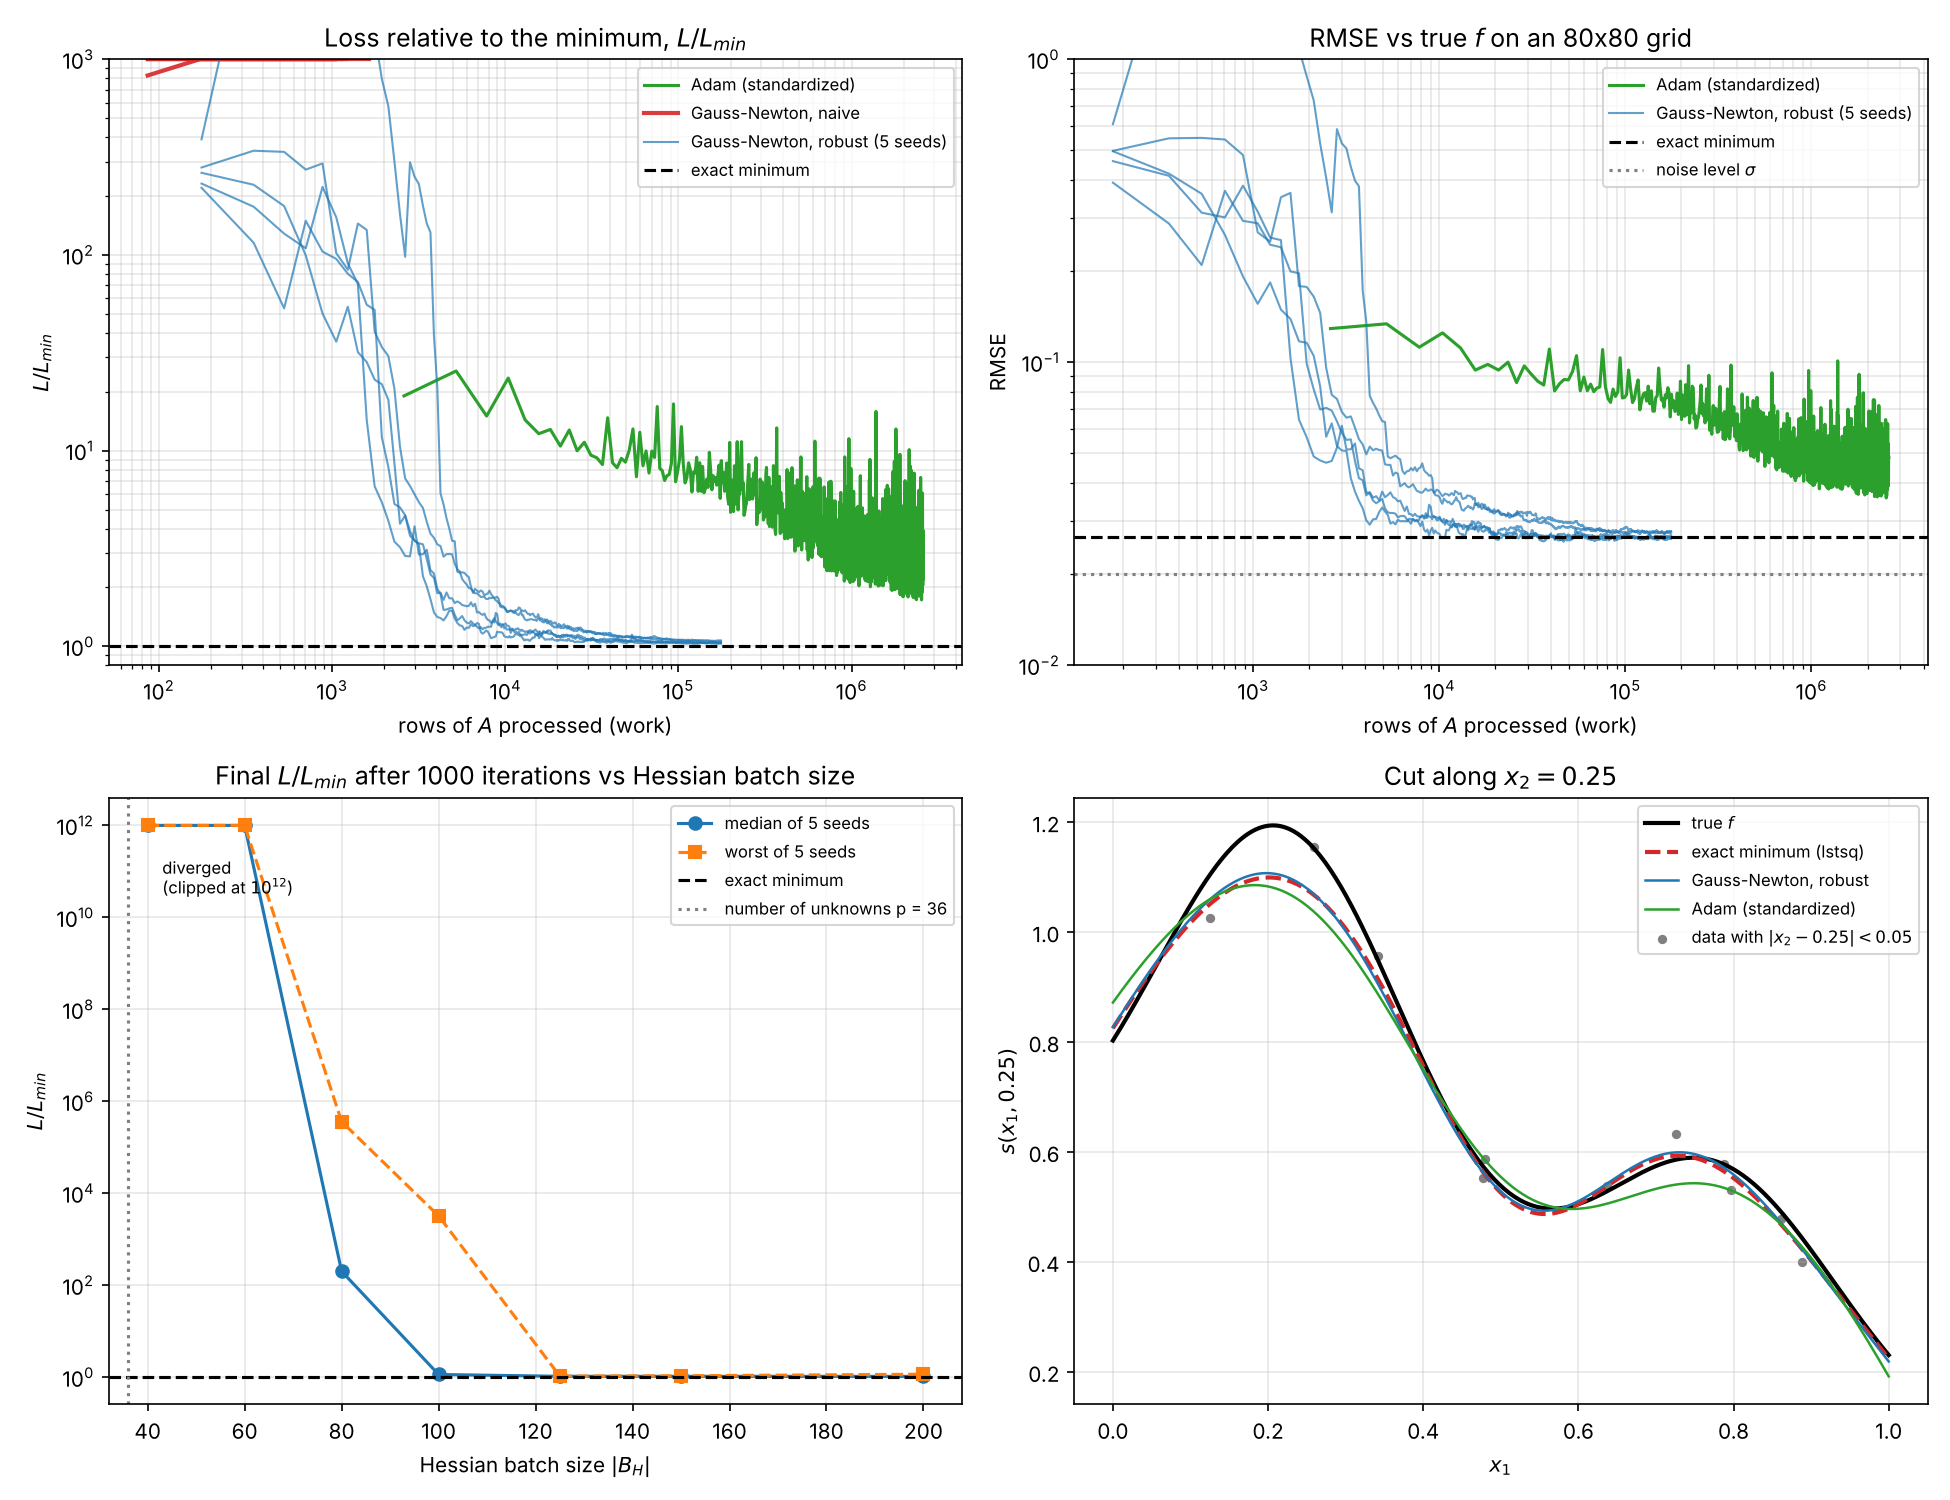
\includegraphics[width=\linewidth,height=0.80\textheight,keepaspectratio,trim=0 359 467 0,clip]{example04_results.png}
    \end{column}
    \begin{column}{0.42\textwidth}
      \begin{itemize}
        \item Horizontal axis: rows of $A$ processed (log scale).
        \item Blue: robust Gauss-Newton, 5 seeds. Green: Adam.
        \item Red (top): naive Gauss-Newton, diverging after a few iterations.
        \item Second order reaches the minimum; first order stalls far above it.
      \end{itemize}
    \end{column}
  \end{columns}
\end{frame}

\begin{frame}{Example 4: how large must the Hessian sample be?}
  \begin{columns}[c]
    \begin{column}{0.56\textwidth}
      \centering
      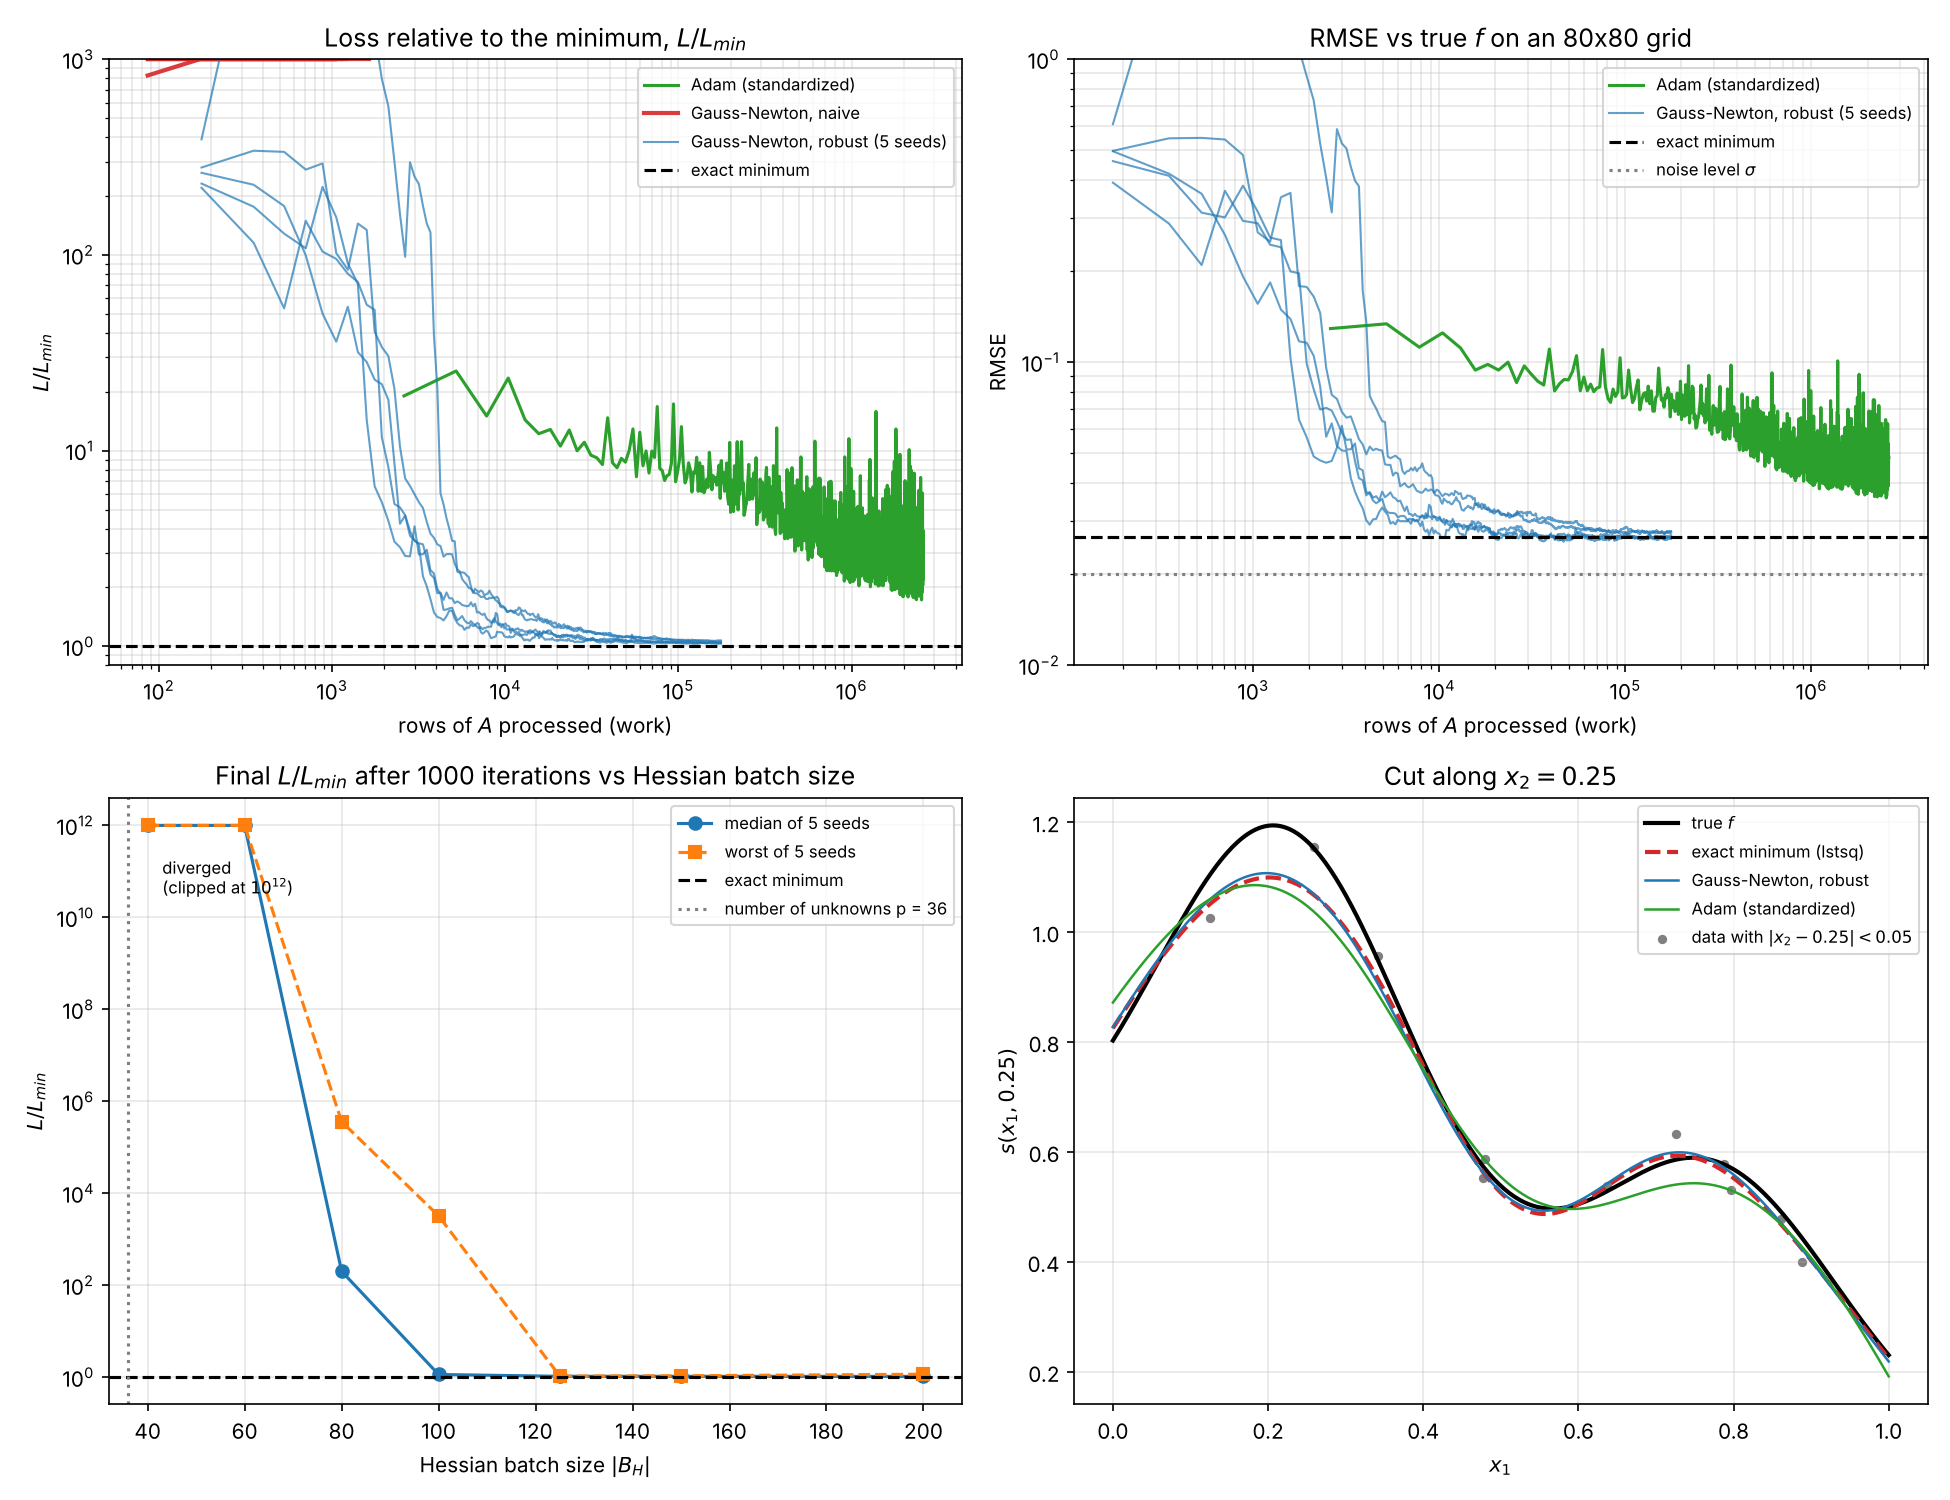
\includegraphics[width=\linewidth,height=0.80\textheight,keepaspectratio,trim=0 0 467 361,clip]{example04_results.png}
    \end{column}
    \begin{column}{0.42\textwidth}
      \begin{itemize}
        \item Final $L/L_{\min}$ after 1000 iterations vs.\ $|B_H|$ (5 seeds).
        \item $|B_H| \le 60$: diverges. $80$--$100$: depends on the seed.
        \item $|B_H| \ge 125$: robust.
        \item The threshold is well above $p = 36$: the flat directions need many rows to be seen correctly.
      \end{itemize}
    \end{column}
  \end{columns}
\end{frame}

\begin{frame}{Example 4: observations}
  \begin{itemize}
    \item \textbf{Curvature breaks the barrier.} Second-order steps are more
          expensive, but hundreds of them replace millions of gradient steps.
    \item \textbf{But it is not free.} The naive version diverges. Robustness
          needs a large enough Hessian sample, damping $\mu$ and a decreasing
          step.
    \item \textbf{An honest caveat.} Here the robust Hessian sample is $75\%$
          of the data, almost the full Hessian. Theory says the needed sample
          size depends on $p$ and on how the information is spread among the
          rows, \emph{not} on $n$. With millions of data it would be a tiny
          fraction, but this small example cannot show that.
  \end{itemize}
  \vspace{0.5em}
  \begin{alertblock}{Question}
    Can we use curvature with mini-batches \emph{smaller} than $p$, even of
    size one?
  \end{alertblock}
\end{frame}

% =====================================================================
\section{Example 5: recursive least squares (Sherman-Morrison)}
% =====================================================================

\begin{frame}{Accumulate the curvature one row at a time}
  To know the curvature in all $p$ directions we need the information of at
  least $p$ independent rows. But it does not have to arrive \hl{in the
  same iteration}: it can be \hl{accumulated}.
  \vspace{0.5em}

  Process the rows one by one, $\bm{a}_1, \bm{a}_2, \dots$, and keep
  \[
    P_k = \big(\delta I + \bm{a}_1\bm{a}_1^T + \cdots + \bm{a}_k\bm{a}_k^T\big)^{-1}
    \qquad (p\times p)
  \]
  \[
    \bm{w}_k = \text{least-squares solution using the first } k \text{ rows}
  \]
  \begin{itemize}
    \item $P_k$ is the inverse Hessian of all the data seen so far.
    \item $P_k$ is \hl{always $p\times p$}: it never grows. Each new row only
          corrects it.
    \item After using a row we can discard it.
  \end{itemize}
\end{frame}

\begin{frame}{The Sherman-Morrison formula}
  Adding a row $\bm{a}$ changes the matrix by a rank-1 term $\bm{a}\bm{a}^T$.
  Its inverse can be updated \hl{without inverting anything}:
  \[
    \big(M + \bm{a}\bm{a}^T\big)^{-1}
    = M^{-1} - \frac{\big(M^{-1}\bm{a}\big)\big(\bm{a}^TM^{-1}\big)}
                    {1 + \bm{a}^TM^{-1}\bm{a}}
  \]
  This gives the \hl{recursive least squares} (RLS) update for a new datum
  $(\bm{a}_i, y_i)$:
  \begin{block}{RLS step, cost $O(p^2)$}
    \vspace{-0.8em}
    \begin{align*}
      \bm{k} &= \frac{P\bm{a}_i}{1 + \bm{a}_i^TP\bm{a}_i}
             && \text{(gain vector)} \\
      \bm{w} &\leftarrow \bm{w} + \bm{k}\,\big(y_i - \bm{a}_i^T\bm{w}\big)
             && \text{(correct with the new residual)} \\
      P &\leftarrow P - \bm{k}\,\big(P\bm{a}_i\big)^T
             && \text{(Sherman-Morrison)}
    \end{align*}
  \end{block}
  A second-order method with mini-batches of size \hl{one}. It is the linear
  case of the Kalman filter.
\end{frame}

\begin{frame}{Practical questions}
  \begin{itemize}
    \item \textbf{How to start?} With fewer than $p$ rows,
          $\sum \bm{a}_i\bm{a}_i^T$ is not invertible. Start with
          $P_0 = I/\delta$, $\delta$ very small (a tiny regularization).
    \item \textbf{When does it end?} After \hl{one pass over all $n$ rows},
          $\bm{w}$ is the solution of
          \[
            \big(A^TA + \delta I\big)\,\bm{w} = A^T\bm{y}
          \]
          i.e.\ least squares with a tiny ridge regularization.
    \item \textbf{All $n$ rows, not just $p$.} With only the first $p$ rows we
          would just fit those $p$ data. $p$ rows is the minimum to make $P$
          well defined; the full approximation needs all $n$.
    \item \textbf{Does the order matter?} Not for the final result: a sum does
          not depend on the order of its terms. It does change the
          intermediate models.
    \item \textbf{Streaming data:} a forgetting factor $0<\lambda_f<1$
          discounts old data; the model ``remembers'' the last
          $\approx 1/(1-\lambda_f)$ rows.
  \end{itemize}
\end{frame}

\begin{frame}{Example 5: results}
  Same problem as Examples 3 and 4, $\delta = 10^{-10}$, one pass.
  \vspace{0.5em}

  \centering
  \begin{tabular}{lccc}
    \toprule
    Method & $L/L_{\min}$ & RMSE vs.\ $f$ & rows processed \\
    \midrule
    \texttt{lstsq} (exact) & 1.000000 & 0.0265 & 206 \\
    \hl{RLS}, rows sorted by $x_1$ & \hl{1.000006} & 0.0265 & \hl{206} \\
    \hl{RLS}, random order & \hl{1.000006} & 0.0265 & \hl{206} \\
    \midrule
    Stochastic Gauss-Newton (Example 4) & 1.04 & 0.027 & $1.8\times10^{5}$ \\
    Adam, standardized (Example 3) & 3.25 & 0.049 & $2.6\times10^{6}$ \\
    \bottomrule
  \end{tabular}
  \vspace{0.8em}

  \raggedright
  \begin{itemize}
    \item One pass, one row at a time, and the \hl{exact} answer.
    \item Sorted and random order give the same final $\bm{w}$ (difference
          $\approx 10^{-4}$, round-off).
  \end{itemize}
\end{frame}

\begin{frame}{Example 5: the model built row by row}
  \begin{columns}[c]
    \begin{column}{0.56\textwidth}
      \centering
      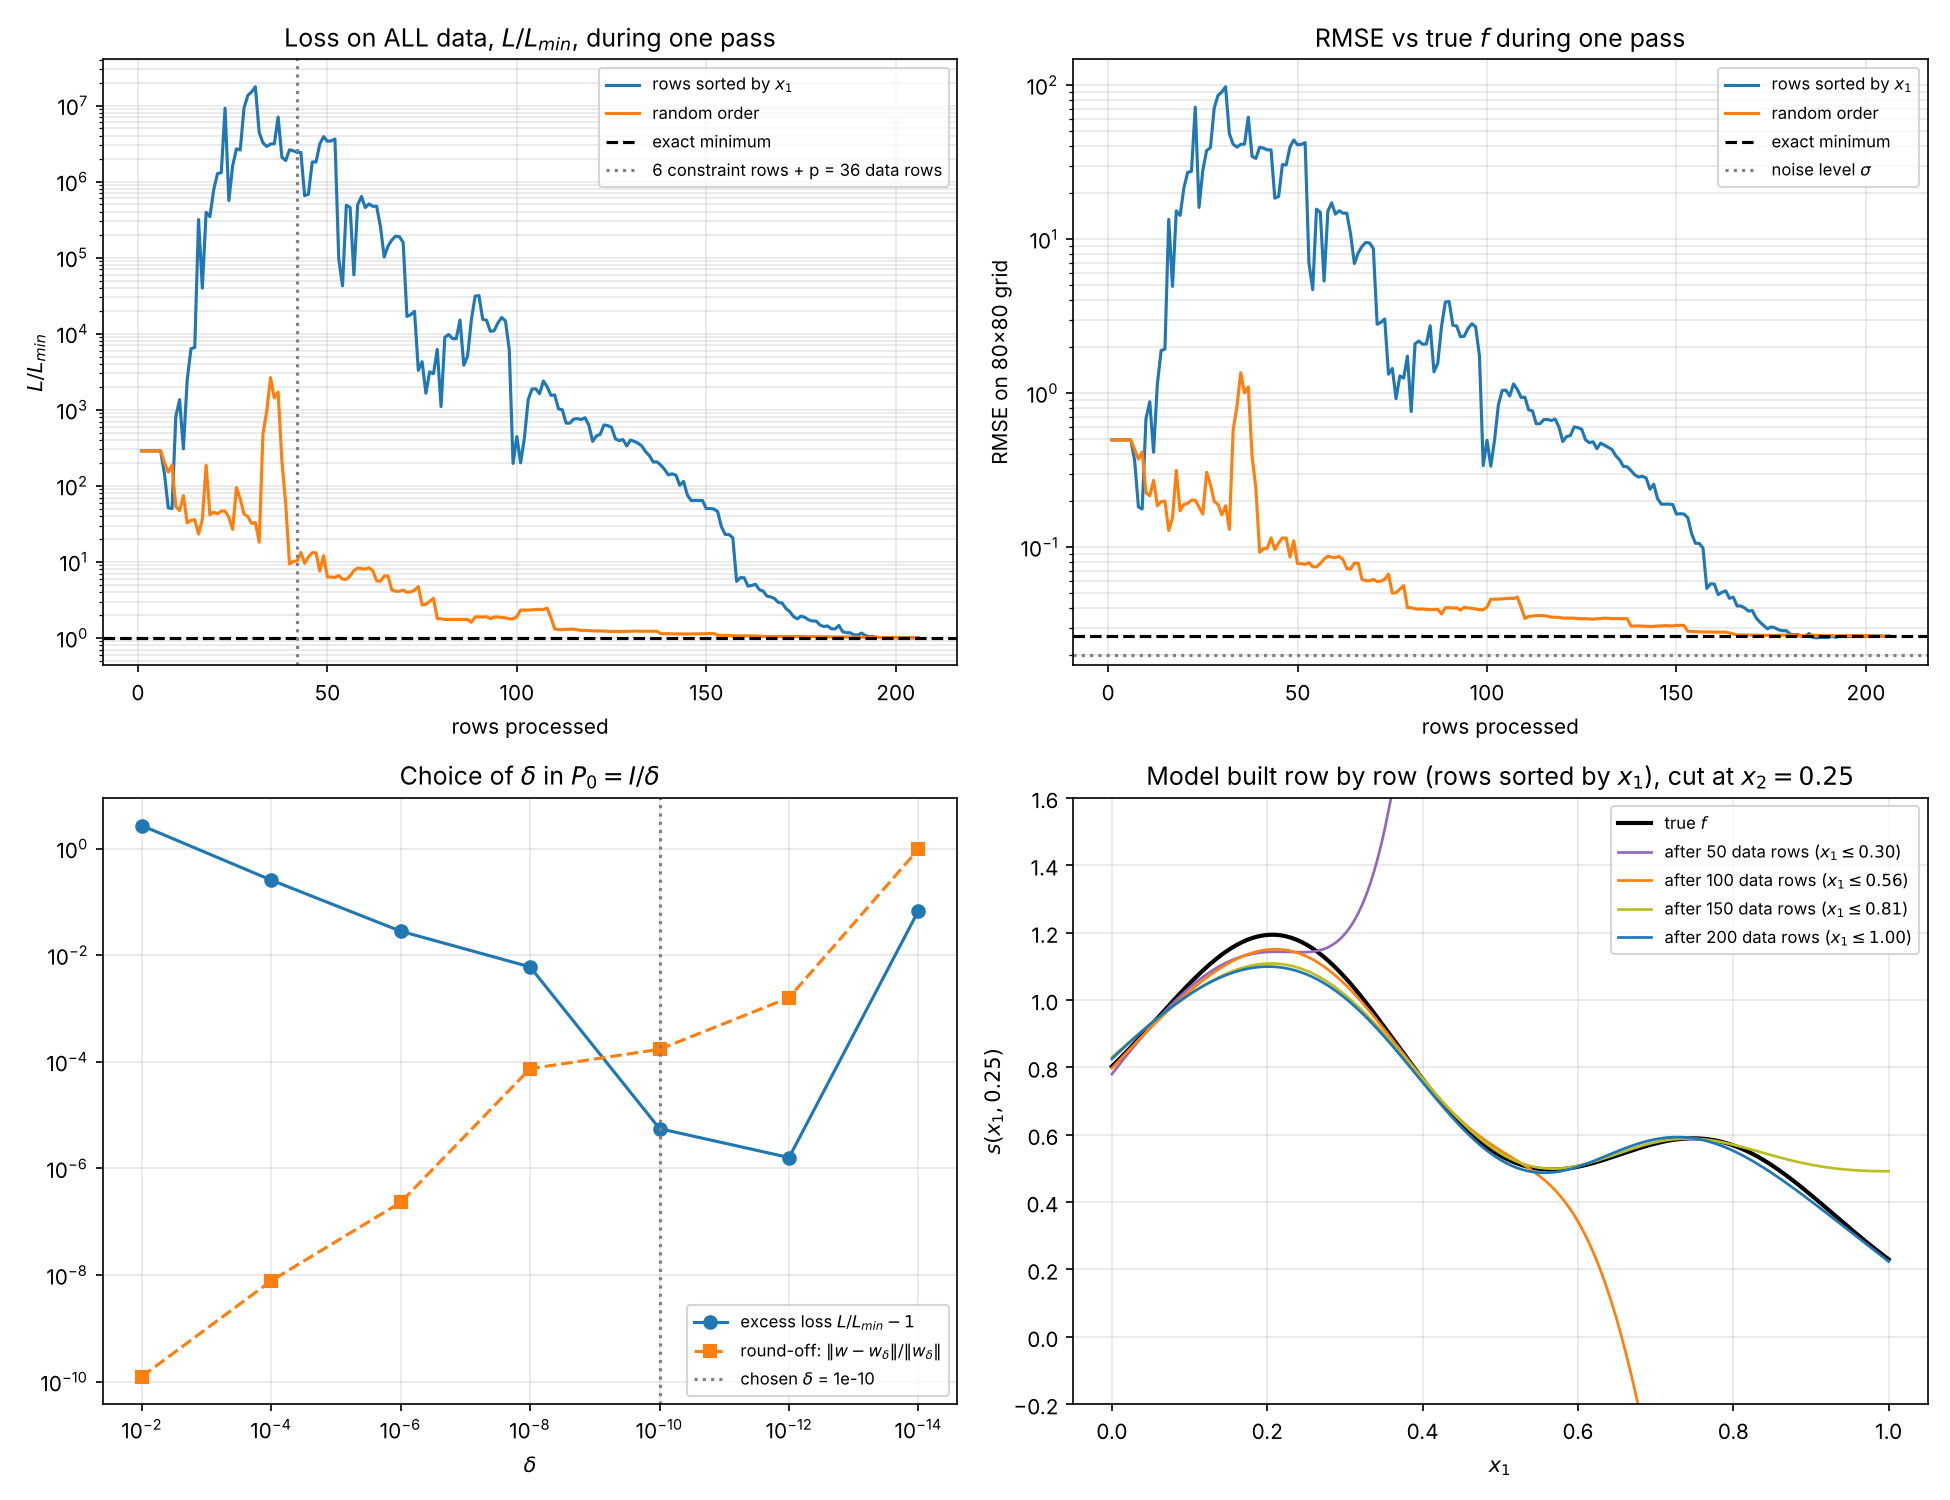
\includegraphics[width=\linewidth,height=0.80\textheight,keepaspectratio,trim=466 0 0 361,clip]{example05_results.png}
    \end{column}
    \begin{column}{0.42\textwidth}
      \begin{itemize}
        \item Rows sorted by $x_1$: the data enter from left to right.
        \item Cut along $x_2 = 0.25$ after 50, 100, 150 and 200 data rows.
        \item The model is good where data have been seen, and wild where they have not.
        \item After all rows: the exact least-squares model.
      \end{itemize}
    \end{column}
  \end{columns}
\end{frame}

\begin{frame}{Example 5: the loss during one pass}
  \begin{columns}[c]
    \begin{column}{0.56\textwidth}
      \centering
      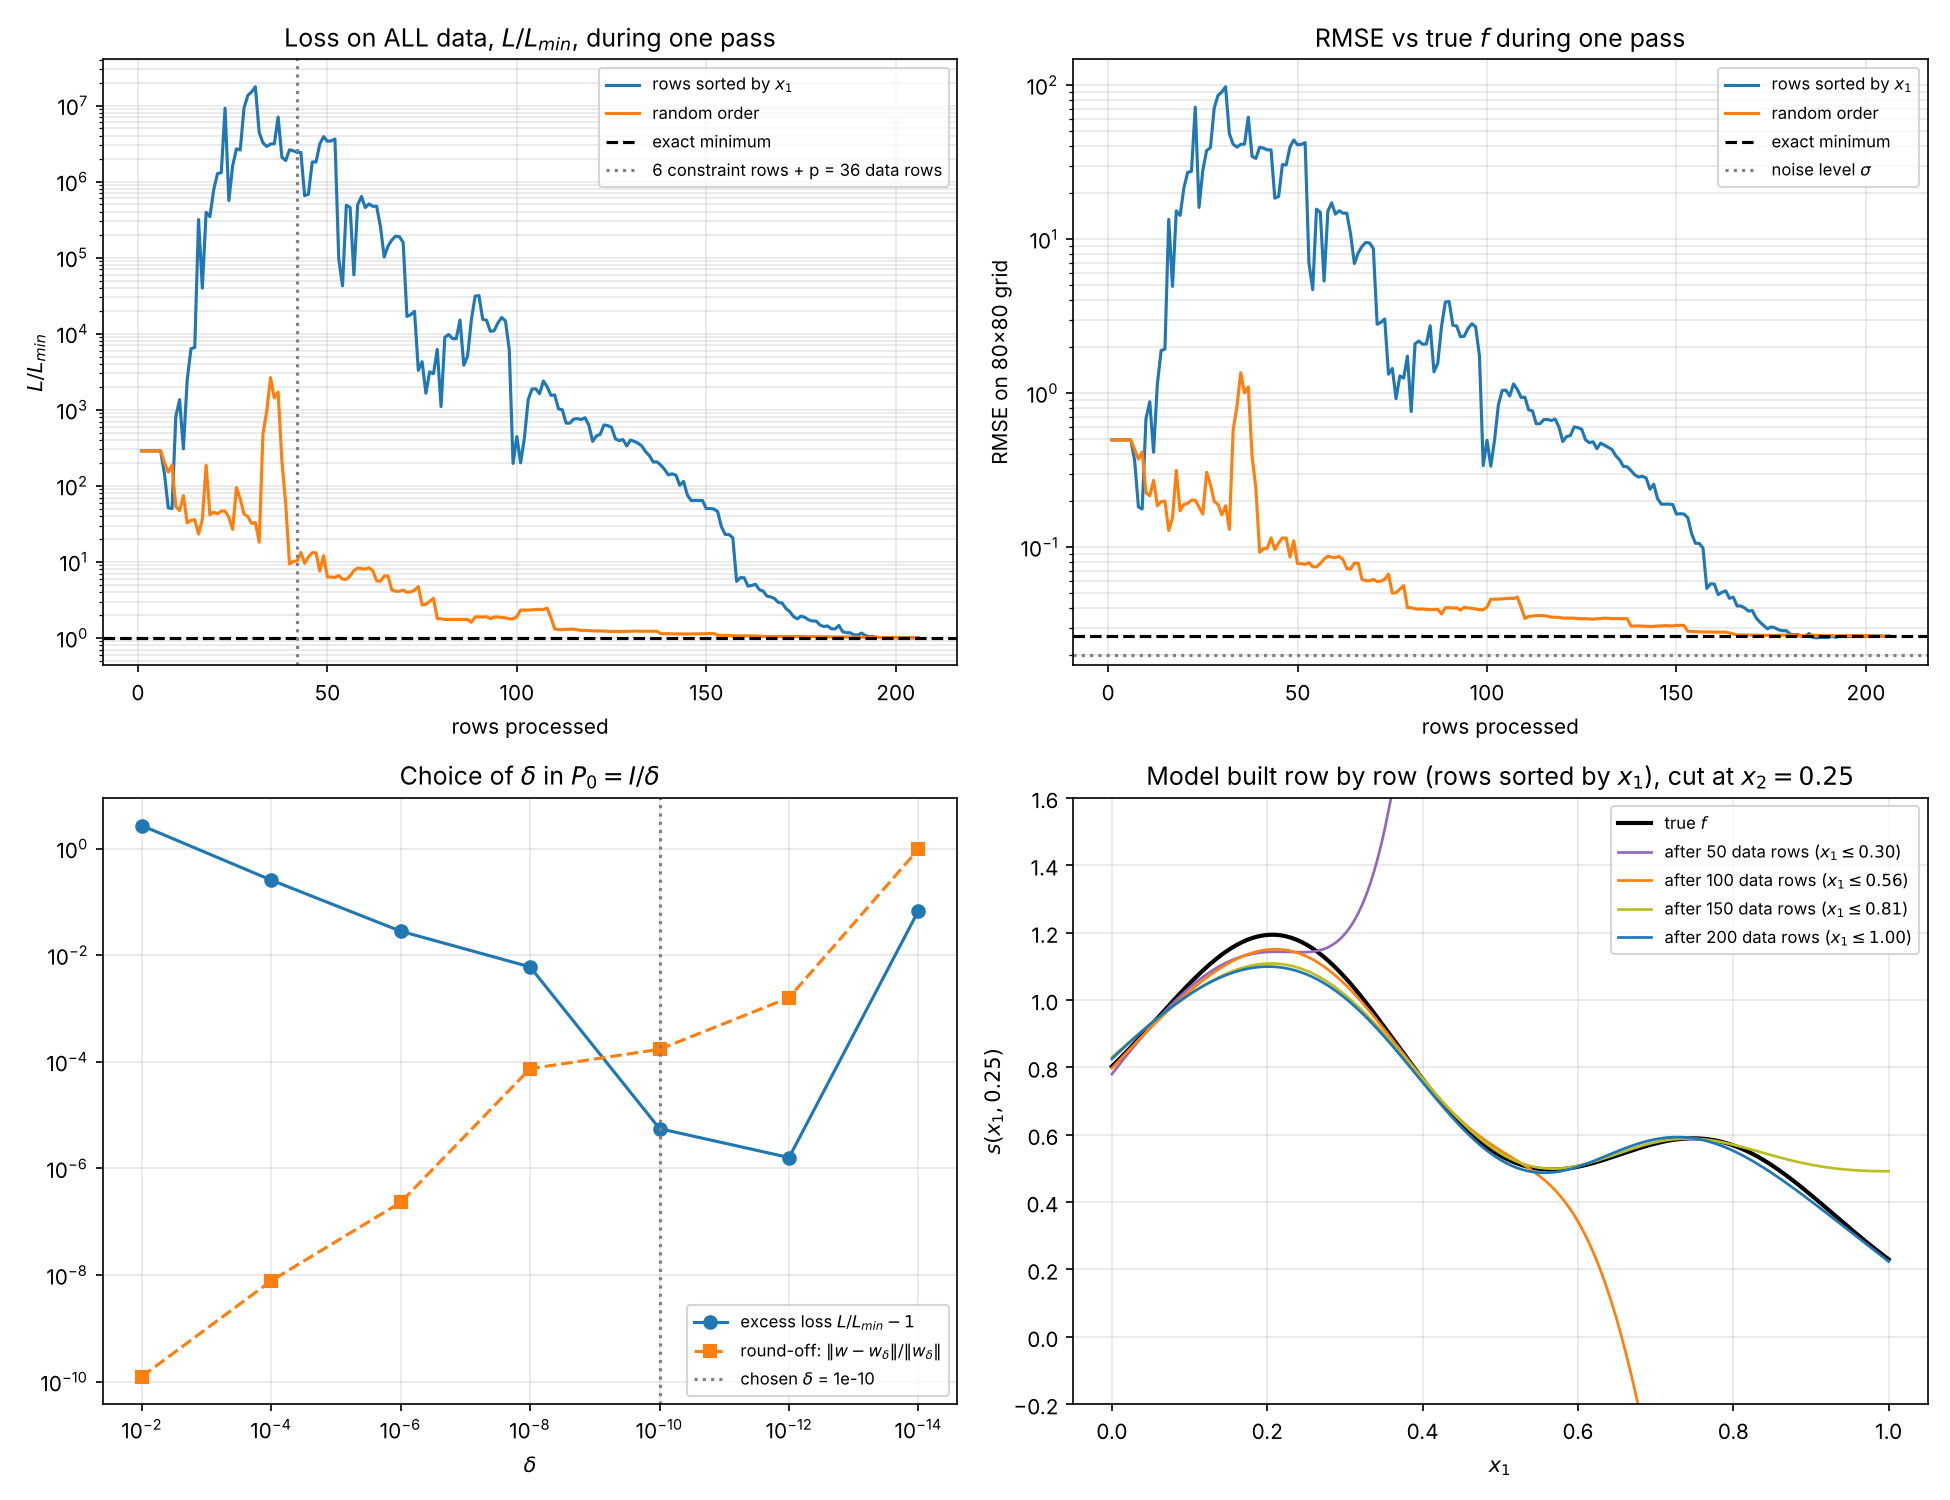
\includegraphics[width=\linewidth,height=0.80\textheight,keepaspectratio,trim=0 359 470 0,clip]{example05_results.png}
    \end{column}
    \begin{column}{0.42\textwidth}
      \begin{itemize}
        \item Loss on \emph{all} data while the rows are being processed.
        \item Sorted order: very large intermediate errors (unseen regions).
        \item Random order: intermediate models are representative much earlier.
        \item Both end exactly at the minimum.
      \end{itemize}
    \end{column}
  \end{columns}
\end{frame}

\begin{frame}{Example 5: choosing $\delta$}
  \begin{columns}[c]
    \begin{column}{0.56\textwidth}
      \centering
      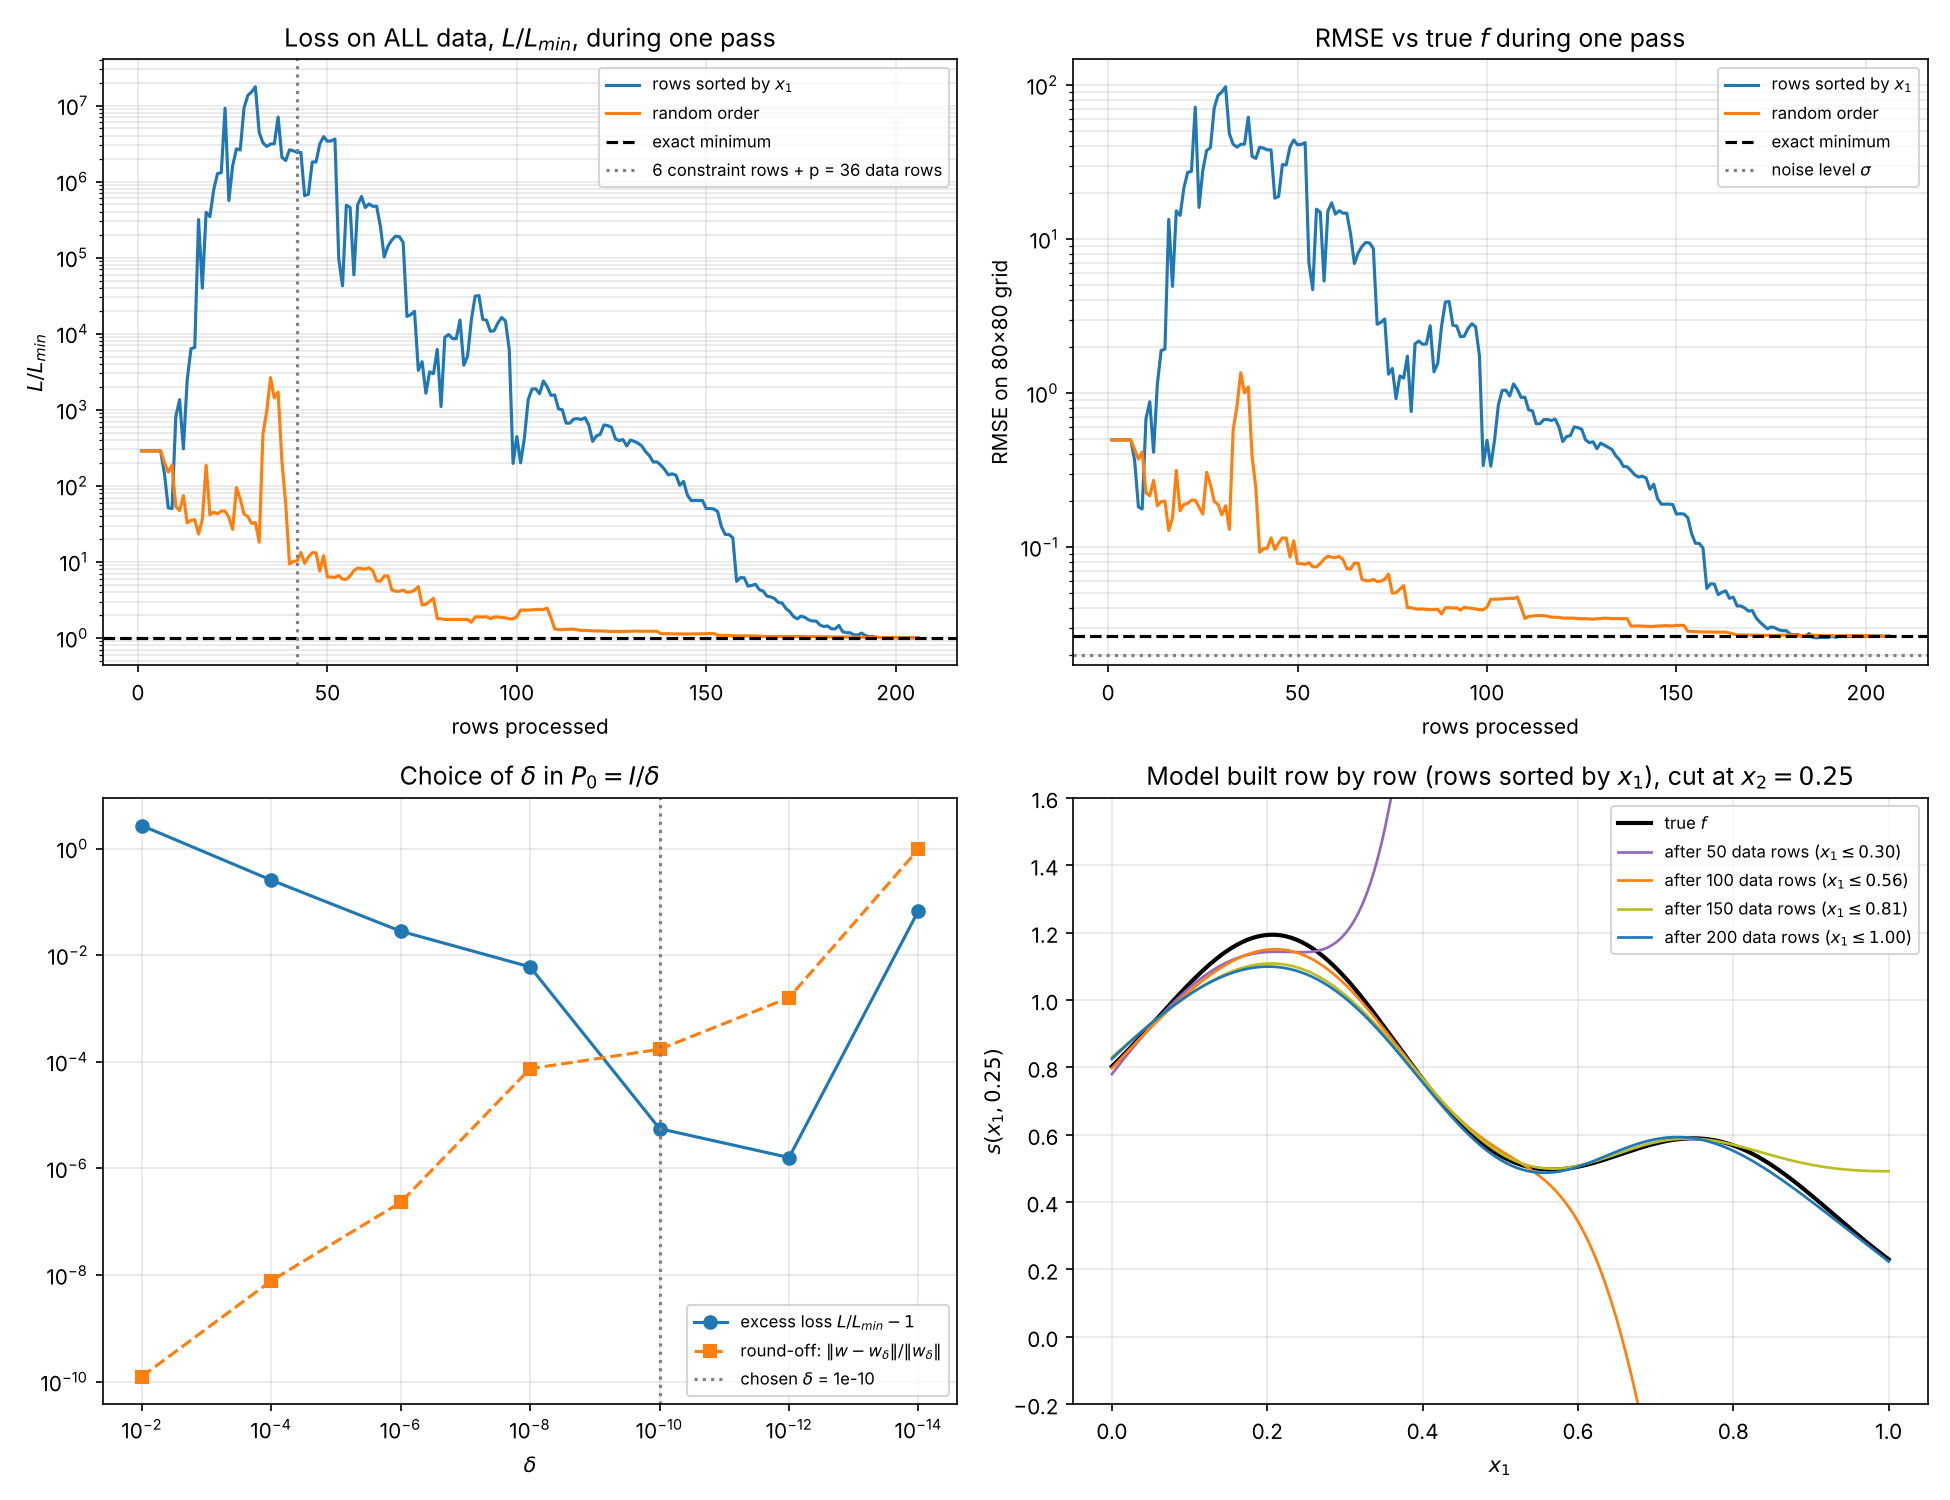
\includegraphics[width=\linewidth,height=0.80\textheight,keepaspectratio,trim=0 0 470 361,clip]{example05_results.png}
    \end{column}
    \begin{column}{0.42\textwidth}
      \begin{itemize}
        \item Large $\delta$: regularization bias (excess loss).
        \item Tiny $\delta$: round-off error grows. RLS works with $A^TA$, whose condition number is $\operatorname{cond}(A)^2 \approx 5\times10^{12}$.
        \item Best compromise here: $\delta \approx 10^{-10}$.
        \item Robust variants exist (QR-based, square-root RLS).
      \end{itemize}
    \end{column}
  \end{columns}
\end{frame}

\begin{frame}{Comparing the five ways of computing the coefficients}
  \centering\small
  \begin{tabular}{llcccc}
    \toprule
    Ex. & Method & Order & Batch & Rows processed & $L/L_{\min}$ \\
    \midrule
    1 & SLSQP, exact constraint & quasi-Newton & all & -- & 1.01 \\
    3 & SGD / momentum / Adam & 1st & 20 & $2.6\times10^{6}$ & $\ge 3.3$ \\
    4 & Stochastic Gauss-Newton & 2nd & 20 / 150 & $1.8\times10^{5}$ & 1.04 \\
    5 & RLS (Sherman-Morrison) & 2nd & 1 & 206 & 1.000006 \\
    -- & \texttt{lstsq} (SVD) & direct & all & 206 & 1 \\
    \bottomrule
  \end{tabular}
  \vspace{0.8em}

  \raggedright
  \begin{itemize}
    \item Small batches and scalability do not require giving up the
          mathematics: RLS processes one datum at a time and is exact.
    \item The real limit is the \hl{conditioning}: it slows down first-order
          methods, and forces care (damping, $\delta$, round-off) in
          second-order ones.
  \end{itemize}
\end{frame}

% =====================================================================
\section{RBF and neural networks}
% =====================================================================

\begin{frame}{Universal approximators}
  \begin{block}{Definition}
    A family of functions $\mathcal{F}$ is a \textbf{universal approximator}
    on a compact set $K\subset\R^d$ if, for every continuous $f$ and every
    $\epsilon>0$, there is $s\in\mathcal{F}$ with
    \[
      \max_{\x\in K} |f(\x) - s(\x)| < \epsilon .
    \]
  \end{block}
  \begin{itemize}
    \item \textbf{Multilayer neural networks:} already one hidden layer with a
          non-polynomial activation is enough (Cybenko 1989; Hornik et al.\
          1989; Leshno et al.\ 1993).
    \item \textbf{RBF:} $\sum_j a_j\phi(\lVert\x-\cc_j\rVert)$ is a universal
          approximator too (Park \& Sandberg 1991). An RBF model \emph{is} a
          one-hidden-layer network with a radial activation.
    \item \hl{Existence only}: the theorems say nothing about how many terms
          are needed, how to compute the coefficients, or how accurate the
          derivatives are.
  \end{itemize}
  \vspace{0.3em}
  \begin{alertblock}{So the real question is}
    Which family gives an accurate, reliable and computable approximation
    for a given problem?
  \end{alertblock}
\end{frame}

\begin{frame}{Why and where RBF are preferable}
  \footnotesize
  \begin{columns}[T]
    \begin{column}{0.49\textwidth}
      \textbf{Advantages}
      \begin{itemize}
        \item \hl{Linear in the coefficients} ($\varepsilon$, centers fixed):
              convex, unique global minimum, robust solvers. Networks are
              non-convex (local minima).
        \item \hl{Meshless}: only distances, scattered points, any geometry
              and dimension.
        \item \hl{Accurate derivatives and differential operators}
              ($\nabla s$, $\Delta s$, \dots): high, even spectral, accuracy
              for smooth $f$.
        \item \hl{Local versions scale to large data}: partition of unity
              (RBF-PU), RBF-FD $\Rightarrow$ sparse matrices, millions of
              points, parallel. Fast multipole methods for global ones.
        \item Error estimates, exact interpolation, few hyperparameters.
      \end{itemize}
    \end{column}
    \begin{column}{0.49\textwidth}
      \textbf{Applications}
      \begin{itemize}
        \item \hl{Meshless PDE solvers} (Kansa, local collocation, RBF-FD):
              heat transfer, elasticity, \hl{CFD}, geosciences.
        \item \hl{CFD and FSI}: mesh deformation, data transfer between
              non-matching meshes.
        \item \hl{Image reconstruction}: inpainting, registration, medical
              imaging.
        \item \hl{Surface reconstruction} from 3D point clouds.
        \item Surrogate models for optimization; geostatistics.
      \end{itemize}
      \vspace{0.3em}
      \textbf{Networks are preferable when} the dimension is very high or
      features must be learned from raw data (classification of images,
      text, audio).
      \vspace{0.2em}

      \textbf{RBF challenge:} ill-conditioning of global methods, mitigated
      by local methods and stable bases.
    \end{column}
  \end{columns}
\end{frame}

% =====================================================================
\section{Exercise: optimizing the shape parameter}
% =====================================================================

\begin{frame}{Exercise: optimize $\varepsilon$}
  In both examples $\varepsilon = 3$ was fixed. Once the centers are chosen,
  $\varepsilon$ can also be tuned.
  \vspace{0.3em}
  \begin{itemize}
    \item The coefficients enter \emph{linearly}, $\varepsilon$
          \emph{nonlinearly} $\Rightarrow$ nested (separable) least squares:
          \begin{itemize}
            \item outer: 1D search over $\varepsilon$
                  (\texttt{scipy.optimize.minimize\_scalar});
            \item inner: for each $\varepsilon$, solve the linear problem for
                  $\bm{w}$ and return the error.
          \end{itemize}
  \end{itemize}
  \textbf{Tasks}
  \begin{enumerate}
    \item Use the greedy centers of Example~2. Plot SSE on the data
          vs.\ $\varepsilon \in [0.5, 10]$.
    \item Plot also the LOOCV error and the RMSE vs.\ the true $f$.
    \item Find the optimal $\varepsilon$ for each curve. Do they agree? Why?
    \item Plot $\operatorname{cond}(A)$ vs.\ $\varepsilon$. What happens for
          small $\varepsilon$?
    \item \emph{Bonus:} alternate center selection and $\varepsilon$
          optimization. Does the set of centers change?
  \end{enumerate}
\end{frame}

% =====================================================================
\section{Summary}
% =====================================================================

\begin{frame}{Take-home messages}
  \small
  \begin{itemize}
    \item RBF approximation: $m < n$ terms, coefficients by
          \hl{least squares}. Only distances are needed: it works for
          scattered data in any dimension.
    \item The \hl{polynomial augmentation} captures smooth trends. The
          orthogonality condition is necessary for interpolation, optional
          for approximation.
    \item \hl{Where} the centers are matters: greedy selection reaches the
          same accuracy with far fewer centers than random selection.
    \item More centers always reduce the error on the data, but not the true
          error: beware of \hl{overfitting}.
    \item The RBF matrix is \hl{ill-conditioned}. First-order (gradient)
          methods cannot overcome that: it is a theorem.
    \item Curvature (second order) does, even with sampling: stochastic
          Gauss-Newton, and recursive least squares (one row at a time,
          exact).
  \end{itemize}
  \vspace{0.3em}
  \small Code: \texttt{example01\_rbf\_mq\_slsqp.py}, \texttt{example02\_rbf\_greedy\_centers.py},
  \texttt{example03\_rbf\_sgd.py}, \texttt{example04\_rbf\_stochastic\_gauss\_newton.py},
  \texttt{example05\_rbf\_rls\_sherman\_morrison.py}
\end{frame}

\end{document}
